%% Template.tex; Solar Physics
%% 
\documentclass[namedreferences]{solarphysics}
%
% spr-sola-addons available options:
%  hyperref      -- loads hyperref.sty with options (pdfborder={0 0 0 },urlcolor=blue,breaklinks)
%  nonatbib      -- do not load natbib.sty (style loads it by default)
%  solaromanenum -- makes enumerated list with roman numerals and a single right-bracket
%  linksfromyear -- puts a link on a year citation (hyperref must be loaded). Loaded by default
%  nolinksfromyear -- suppress  linksfromyear
%  optionalrh    -- for optional running title/author
%  showbiblabels -- to show bibitem label at end of bibitem (via \endbibitem command)
%
\usepackage[hyperref,optionalrh,solaromanenum]{spr-sola-addons} % For Solar Physics 
%\usepackage{epsfig}                     % For eps figures, old commands
\usepackage{graphicx}                    % For eps figures, newer & more powerfull
%\usepackage{courier}                    % Change the \texttt command to courier style
\usepackage{amssymb}                    % useful mathematical symbols
\usepackage{color}                       % For color text: \color command
\usepackage{breakurl}                         % For breaking URLs easily trough lines
\def\UrlFont{\sf}                        % define the fonts for the URLs
\usepackage{comment}
\usepackage{setspace}

%% Local definitions
%% please place your own definitions here and don't use \def but
%% \newcommand{}{} or 
%% \renewcommand{}{} if it is already defined in LaTeX
\renewcommand{\deg}{$^\circ$}
\newcommand{\mdeg}{^\circ}
\newcommand{\rsun}{R{$_\odot$}}
\renewcommand{\l}{\lambda_{\rm N}}%\lambda_
\newcommand{\mrsun}{{\rm R_\odot}}
\newcommand{\med}{{\rm Md}}
\newcommand{\avgTe}{\left<T_\textrm{m}\right>}
\newcommand{\MK}{{\rm MK}}
\newcommand{\cm}{{\rm cm}}
\newcommand{\sdev}{{\rm SD}}
\newcommand{\mean}{{\rm Mn}}
\newcommand{\deltat}{$\delta$}
\newcommand{\LDEM}{{\rm LDEM}}
\newcommand{\FBE}{{\rm FBE}}
\newcommand{\TRF}{{\rm TRF}}
\newcommand{\lN}{\lambda_N}
\newcommand{\NCB}{N_{\rm CB}}
\newcommand{\aTm}{\left< T_\textrm{m}\right>}
\newcommand{\Nqi}{N_{\rm QI}}

\newcommand{\Tefit}{T_{e,{\rm fit}}}

\newcommand{\BibTeX}{\textsc{Bib}\TeX}
\newcommand{\etal}{{\it et al.}}


%%%%%%%%%%%%%%%%%%%%%%%%%%%%%%%%%%%%%%%%%%%%%%%%%%%%%%%%%%%%%%%%%%
\begin{document}

\begin{article}

\begin{opening}

\title{Thermodynamic Structure of the Solar Corona: Tomographic Reconstructions and MHD Modeling}

%%%%%%%%%%%%%%%%%%%%%%%%%%%%%%%%%%%%%%%%%%%%%%%%%%%
%% Authors Names
%
% \author[addressref={},corref,email={}]{\inits{}\fnm{}\lnm{}\orcid{}}
\author[addressref={aff1,aff2},corref,email={dlloveras@iafe.uba.ar}]{\inits{D.G.}\fnm{Diego G.}~\lnm{Lloveras}\orcid{0000-0003-1402-0398}}

\author[addressref={aff1,aff3,aff2},corref,email={albert@iafe.uba.ar}]{\inits{A.M.}\fnm{Alberto M.}~\lnm{V\'asquez}\orcid{0000-0003-3401-6409}} 

\author[addressref={aff1,aff2},corref,email={federico@iafe.uba.ar}]{\inits{F.A.}\fnm{Federico A.}~\lnm{Nuevo}\orcid{0000-0003-2355-5853}} 

\author[addressref={},corref,email={nishthas@umich.edu}]{\inits{N.}\fnm{Nishtha}\lnm{Sachdeva}\orcid{1}}

\author[addressref={},corref,email={chipm@umich.edu}]{\inits{W.}\fnm{Ward}\lnm{Manchester IV}\orcid{2}}

\author[addressref={},corref,email={bartvand@umich.edu}]{\inits{B.}\fnm{Bartholomeus}\lnm{Van der Holst}\orcid{3}}

\author[addressref={aff4},corref,email={rfrazin@umich.edu}]{\inits{R.A.}\fnm{Richard A.}~\lnm{Frazin}\orcid{0000-0002-0281-7677}}

%%%%%%%%%%%%%%%%%%%%%%%%%%%%%%%%%%%%%%%%%%%%%%%%%%%
%% Runningheads
%
\runningauthor{D.G.~Lloveras~\etal}
%\runningtitle{}


%%%%%%%%%%%%%%%%%%%%%%%%%%%%%%%%%%%%%%%%%%%%%%%%%%%
%% Affilations 
%% id shold be the same with \author addressref value.
%\address[id={}]{}
\address[id=aff1]{Instituto de Astronom\'{\i}a y F\'{\i}sica del Espacio (IAFE), CONICET-UBA, CC 67 - Suc 28,  (C1428ZAA) Ciudad Aut\'onoma de Buenos Aires, Argentina}

\address[id=aff2]{Departamento de F\'{\i}sica, Facultad de Ciencias Exactas y Naturales (FCEN), Universidad de Buenos Aires (UBA), Pabell\'on I, Ciudad Universitaria, (C1428ZAA) Ciudad Aut\'onoma de Buenos Aires, Argentina}

\address[id=aff3]{Departamento de Ciencia y Tecnolog\'{\i}a, Universidad Nacional de Tres de Febrero (UNTREF), Valent\'{\i}n G\'omez 4752, (B1678ABH) Caseros, Provincia de Buenos Aires, Argentina}

\address[id=aff4]{Department of Climate and Space Sciences and Engineering (CLaSP), University of Michigan, 2455 Hayward Street, Ann Arbor, MI 48109-2143, USA}
%%%%%%%%%%%%%%%%%%%%%%%%%%%%%%%%%%%%%%%%%%%%%%%%%%%
%%% Abstract 
\begin{abstract}
Observational tools play an essential role in advancing our understanding of the physics of the solar corona. They provide validation data to improve three-dimensional (3D) magnetohydrodynamic (MHD) models of the solar atmosphere, key to enhance their space weather forecasting capabilities. Solar rotational tomography (SRT) is currently the sole observational technique that provides an empirical 3D description of fundamental plasma parameters of the solar corona at a global scale. Based on EUV data of space borne instruments, SRT allows constructing 3D maps of the coronal electron density and temperature at heliocentric heights below 1.25 Rsun. We carry out a study of the corona combining tomographic reconstructions with MHD simulations of the latest version of the Alfvén Wave Solar Model (AWSoM) of the Space Weather Modeling Framework (SWMF). Target rotations were selected from the solar minimum between solar cycles (SC) 23 and 24 and the current declining phase of solar cycle 24. Tomographic reconstructions and results of the model are analyzed in distinct coronal magnetic structures. We study magnetically closed structures associated with the equatorial streamer belt, as well as magnetically open regions enclosing it. We report on the tomographic results in the different structures, their implications for the physics of the solar corona, and the capability of the AWSoM model to reproduce the tomographic reconstructions in different regions.

\end{abstract}



%%%%%%%%%%%%%%%%%%%%%%%%%%%%%%%%%%%%%%%%%%%%%%%%%%%
%% Keywords
%
\keywords{Solar Cycle, Observations; Corona,E; Corona, Structures}


\end{opening}
%-------------------------------------------------

%%%%%%%%%%%%%%%%%%%%%%%%%%%%%%%%%%%%%%%%%%%%%%%%%%%
%% Sections
\section{Introduction}\label{intro} 

\section{Methodology}\label{meto}   

\subsection{DEMT reconstructions}\label{demt} 

\subsection{AWSoM simulations}\label{awsom} 

\subsection{Tracing results along fieldlines}\label{trace} 



\section{Results}\label{resu} 
\subsection{Tomographic Results}\label{demt_res} 
A) Carrington (Lat/Lon) maps of the DEMT products Ne and Te at selected heights 1.025, 1.105, 1.205 Rsun, over plotting the Open/Closed (O/C) boundary from the AWSoM model. This plot gives initial CONTEXT.

\begin{figure}%[ht!]
\begin{center}
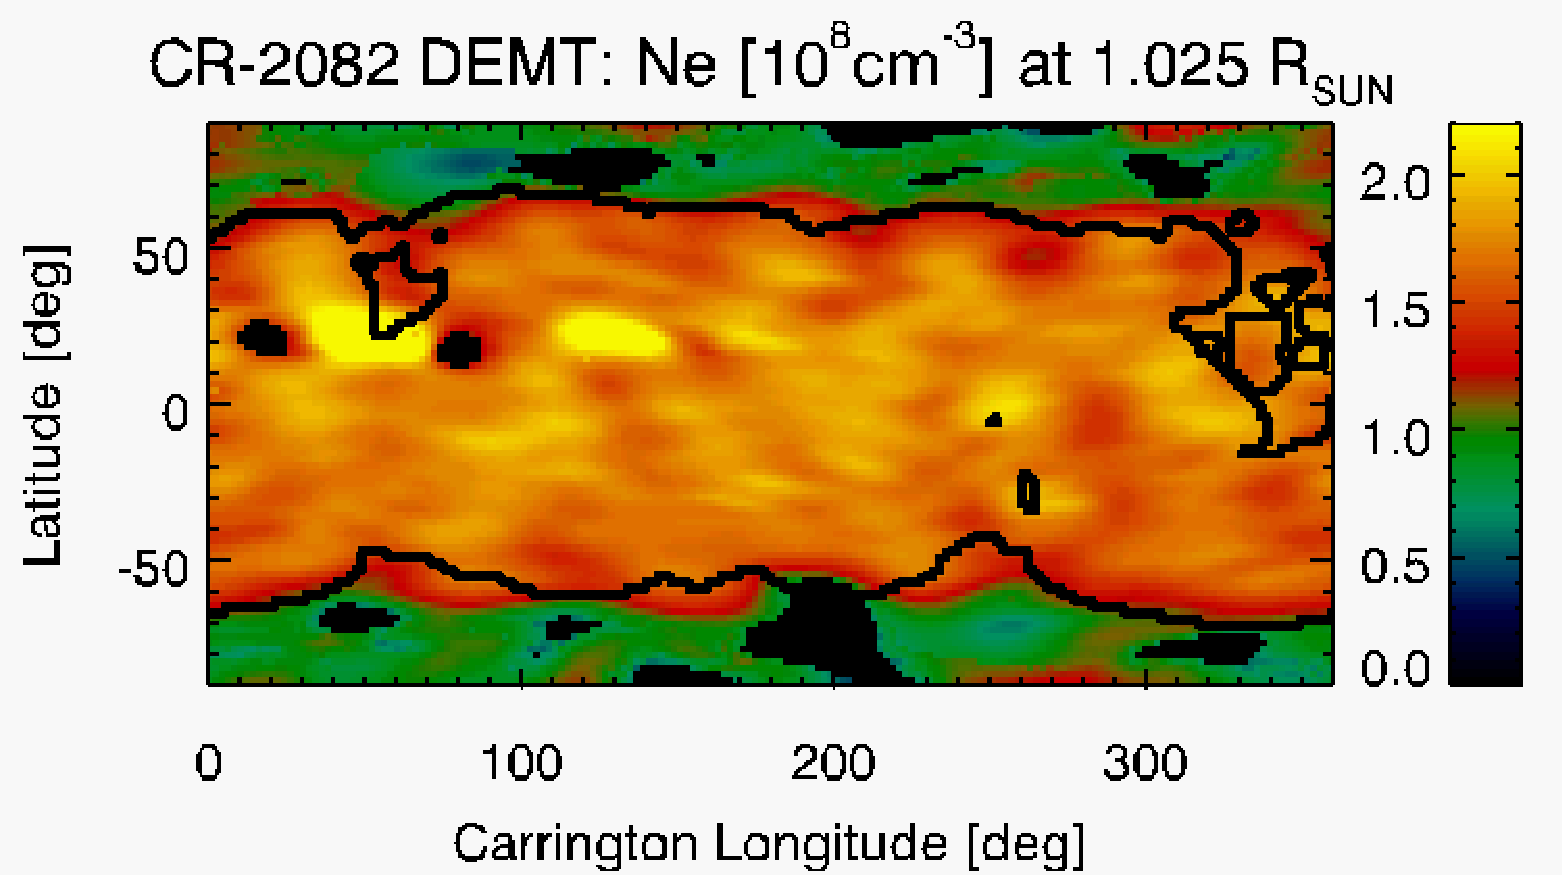
\includegraphics[width=0.495\textwidth]{figs/map_Ne_CR2082_DEMT-EUVI_behind_H1-L3523_r3d_1025_Rsun.pdf}
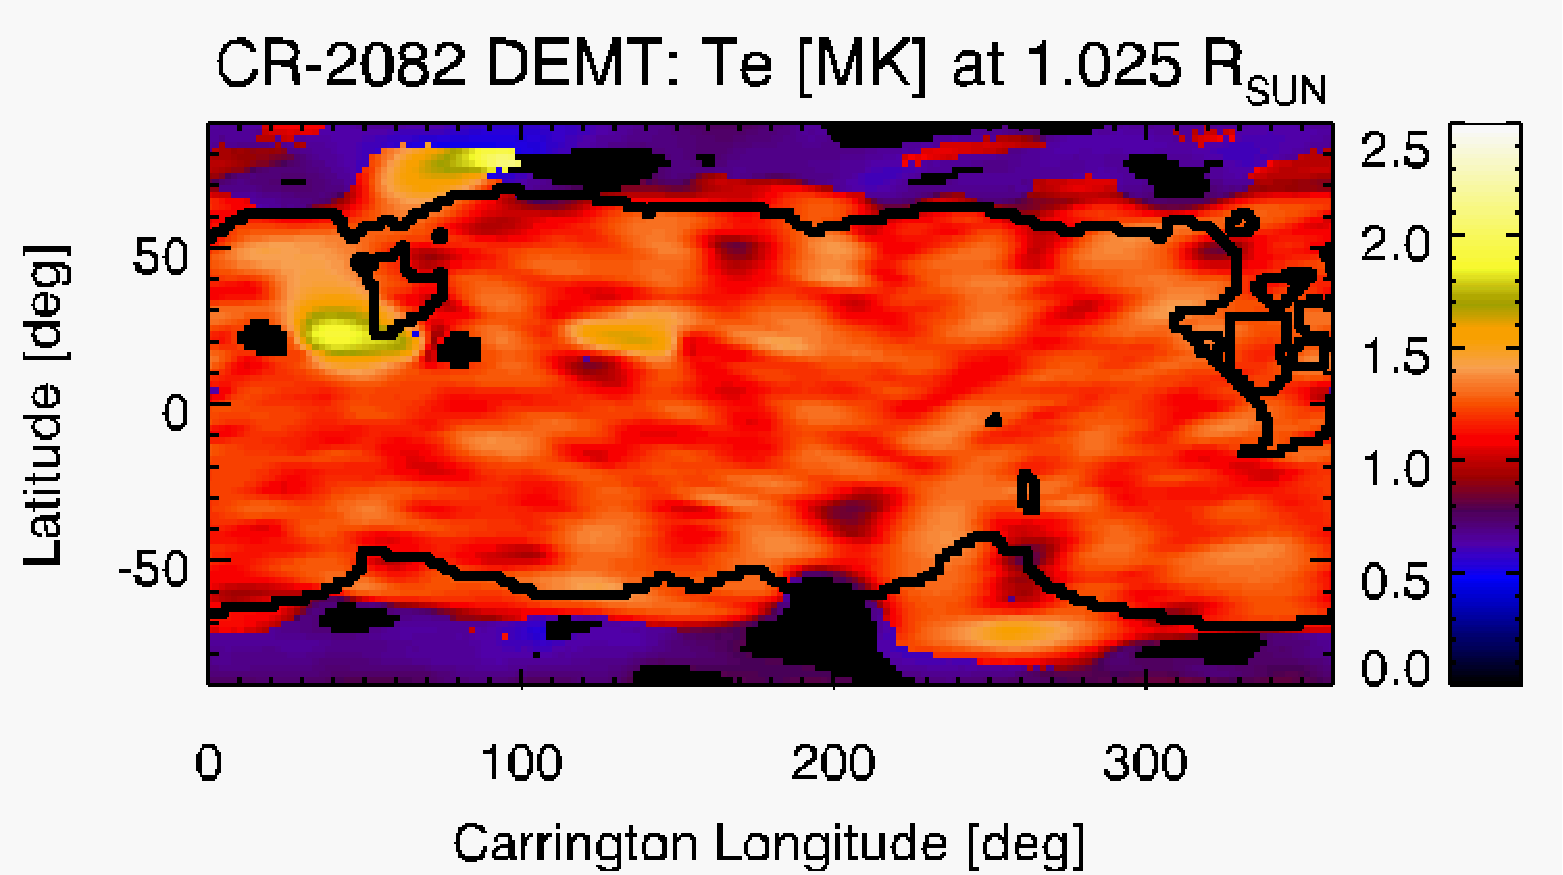
\includegraphics[width=0.495\textwidth]{figs/map_Tm_CR2082_DEMT-EUVI_behind_H1-L3523_r3d_1025_Rsun.pdf}
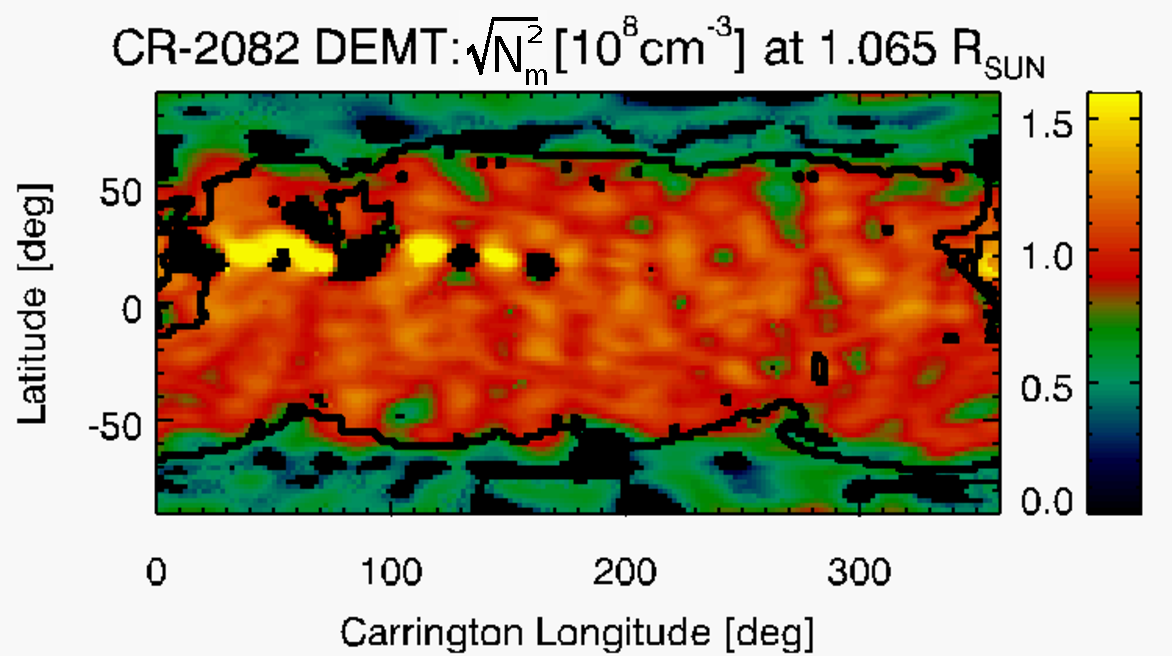
\includegraphics[width=0.495\textwidth]{figs/map_Ne_CR2082_DEMT-EUVI_behind_H1-L3523_r3d_1065_Rsun.pdf}
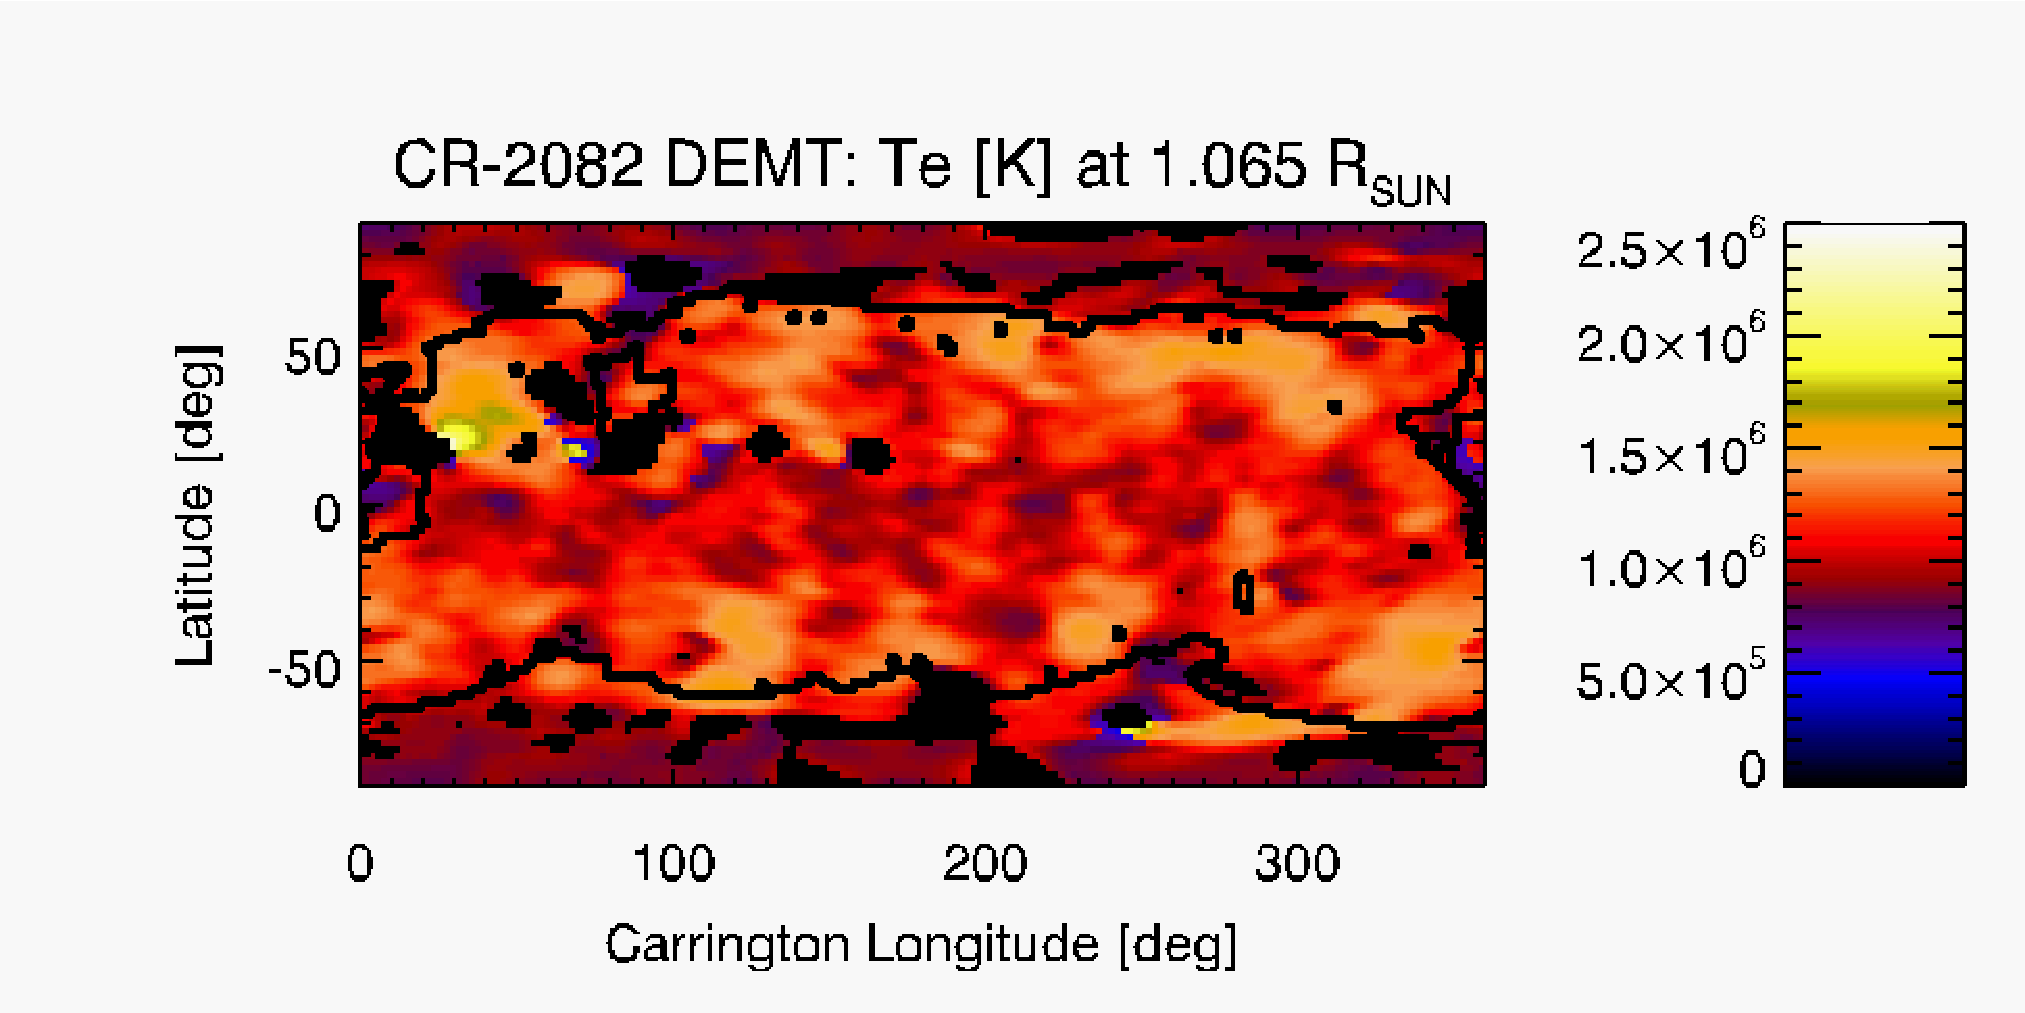
\includegraphics[width=0.495\textwidth]{figs/map_Tm_CR2082_DEMT-EUVI_behind_H1-L3523_r3d_1065_Rsun.pdf}
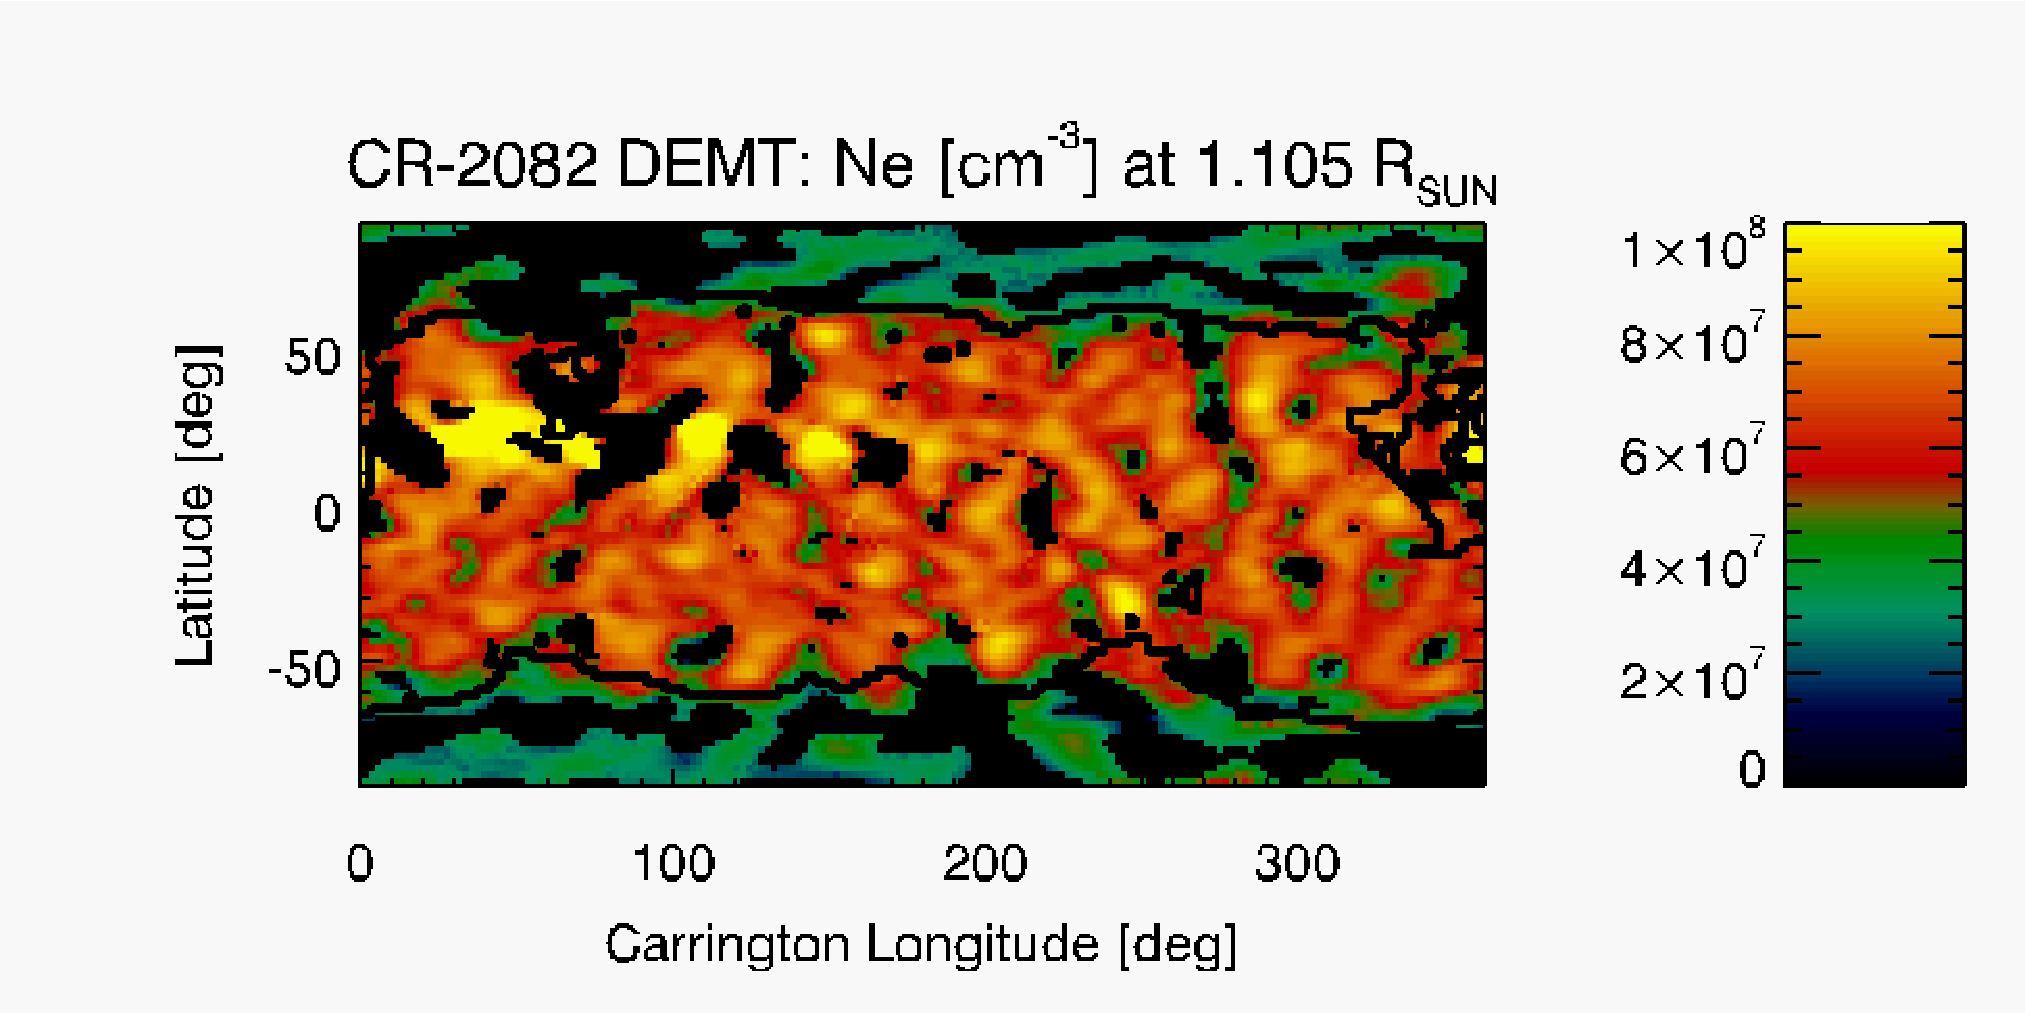
\includegraphics[width=0.495\textwidth]{figs/map_Ne_CR2082_DEMT-EUVI_behind_H1-L3523_r3d_1105_Rsun.pdf}
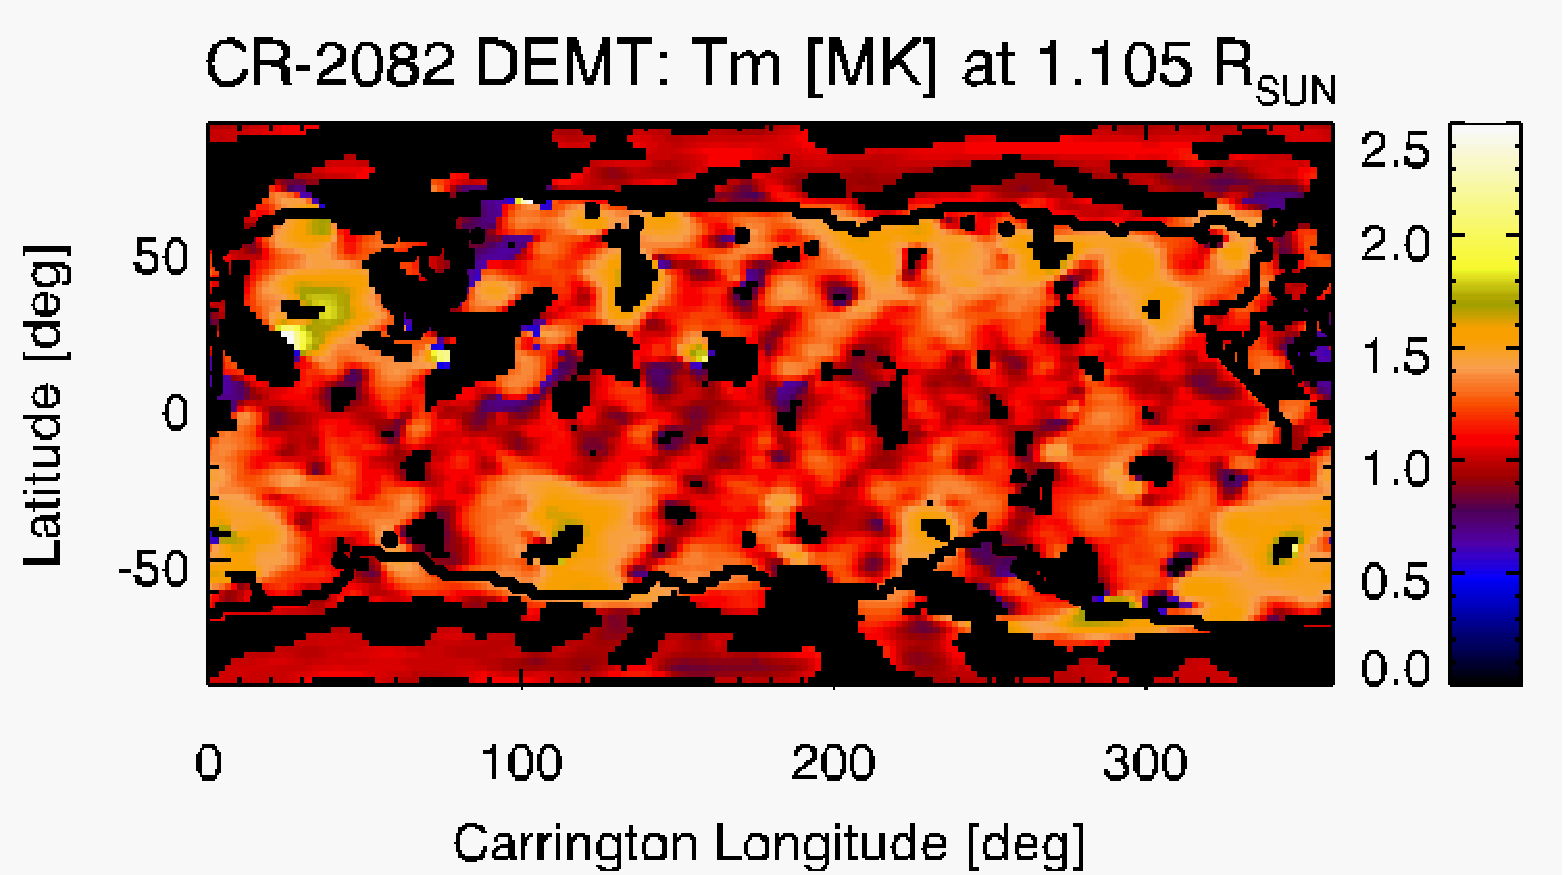
\includegraphics[width=0.495\textwidth]{figs/map_Tm_CR2082_DEMT-EUVI_behind_H1-L3523_r3d_1105_Rsun.pdf}
\caption{Carrington maps of DEMT results: $N_e$ (left panels) and $T_\textrm{m}$ (right panels) for CR-2082. Top, middle and bottom panels show the results at three heliocentric heights, $1.025$ ,$1.065$ $1.105\,\mrsun$, respectively. Black voxels correspond to non-reconstructed regions and thick-black curves indicate the open/closed boundaries.}
\label{carmaps_demt_2082}
\end{center}
\end{figure}

\begin{figure}%[ht!]
\begin{center}
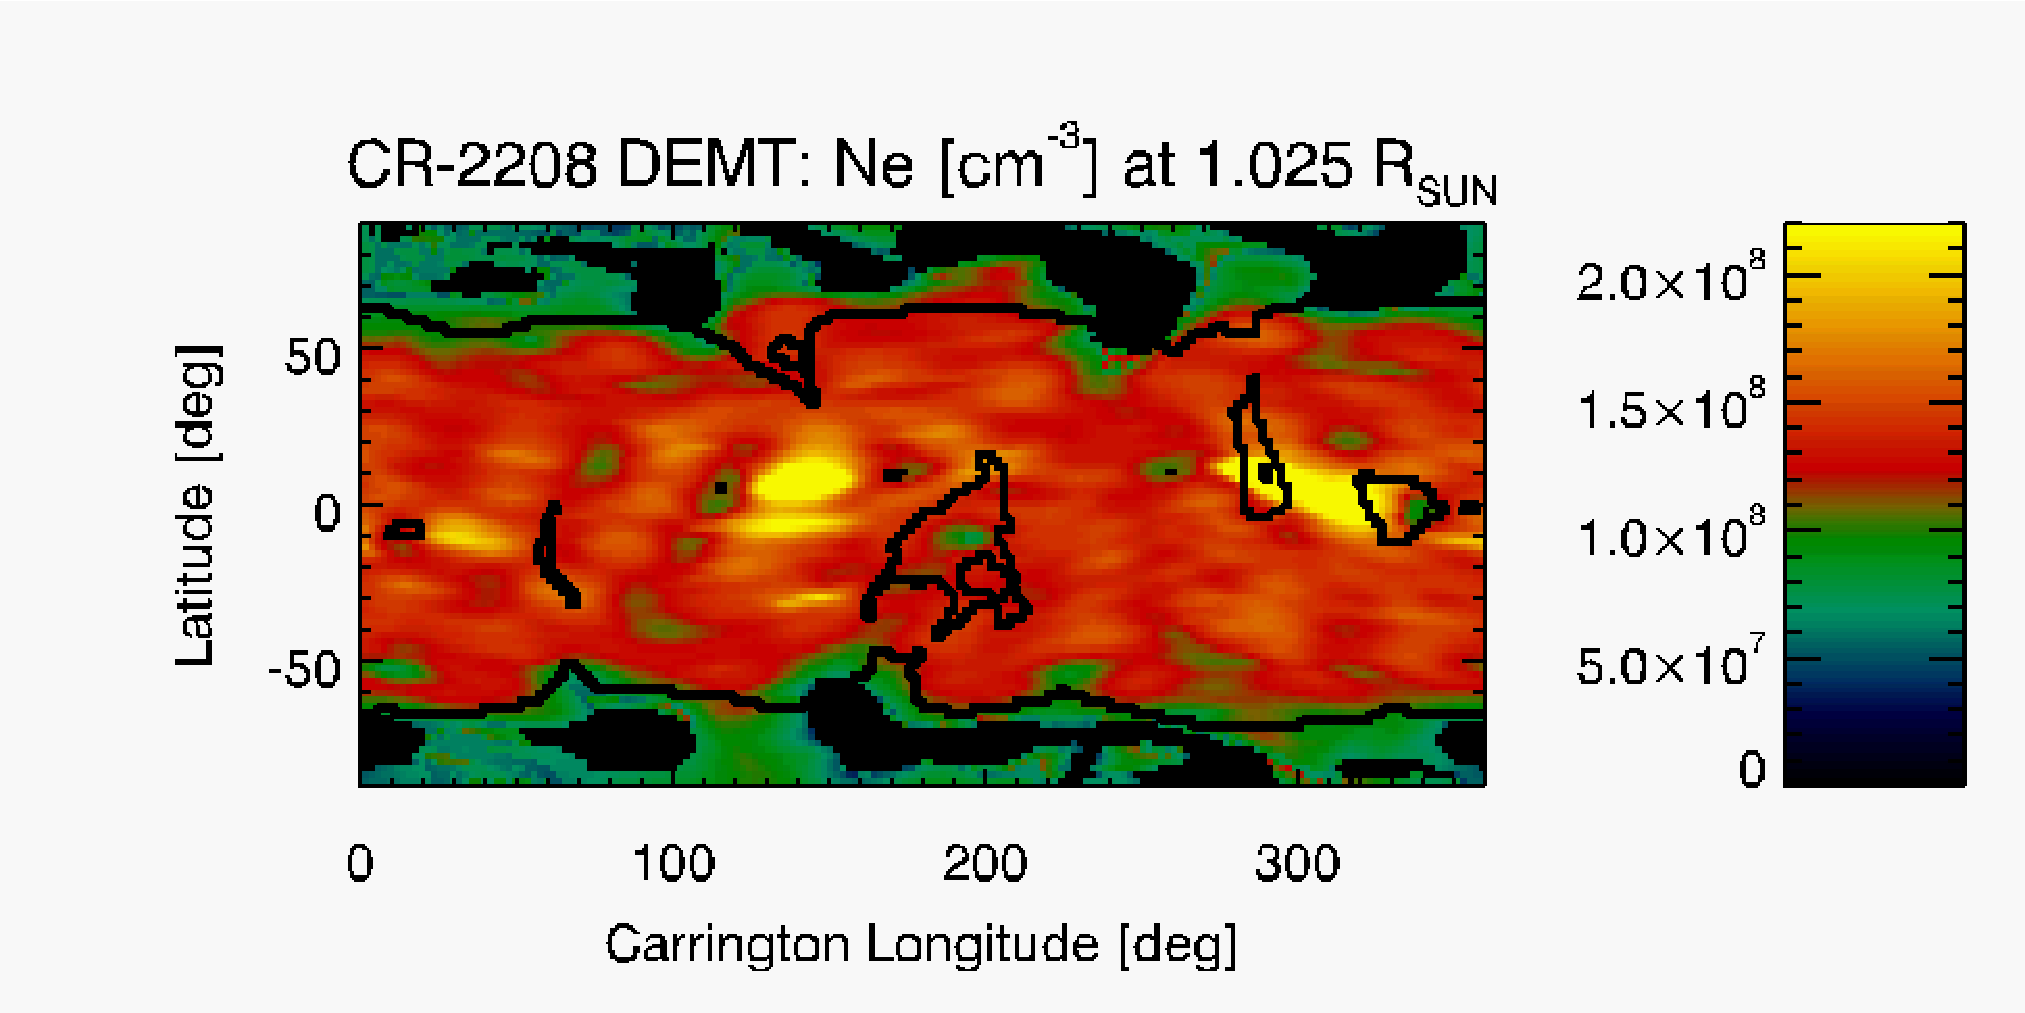
\includegraphics[width=0.495\textwidth]{figs/map_Ne_CR2208_DEMT-AIA_H1_L522_r3d_1025_Rsun.pdf}
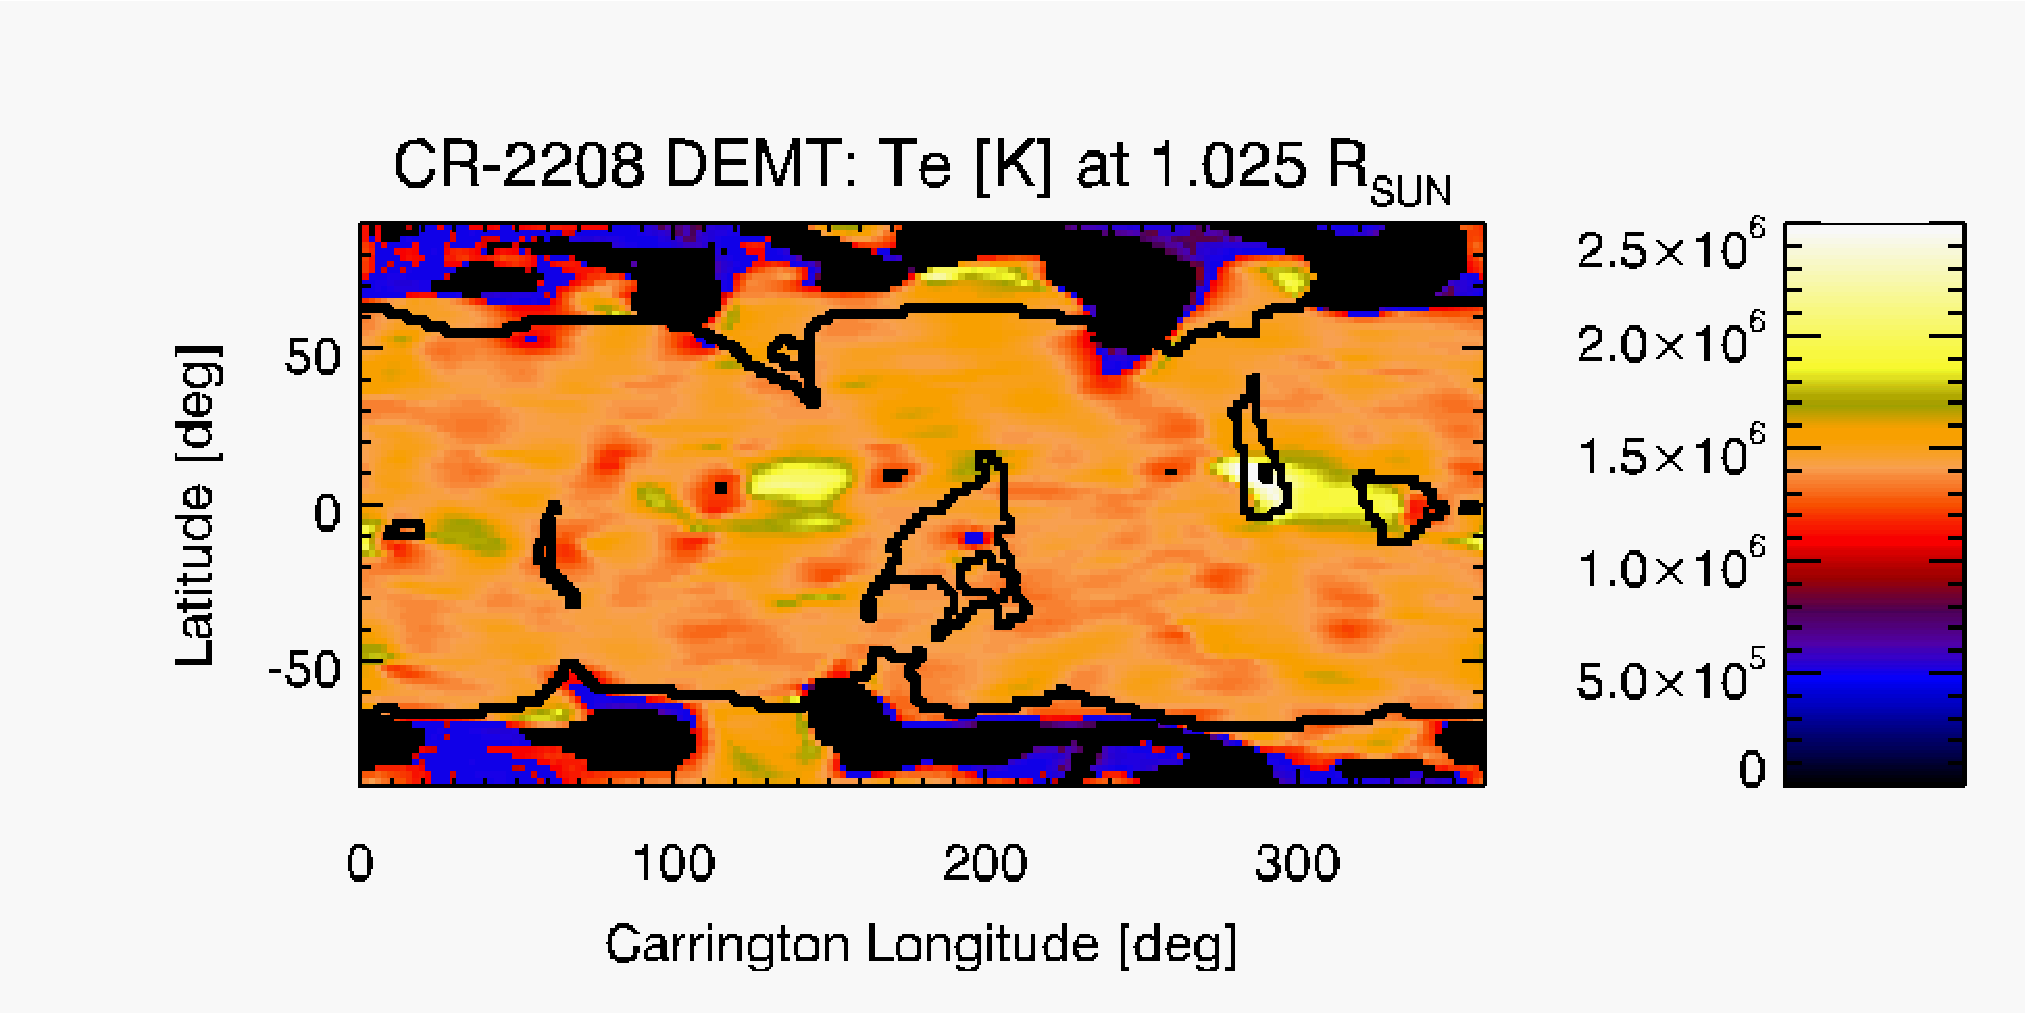
\includegraphics[width=0.495\textwidth]{figs/map_Tm_CR2208_DEMT-AIA_H1_L522_r3d_1025_Rsun.pdf}
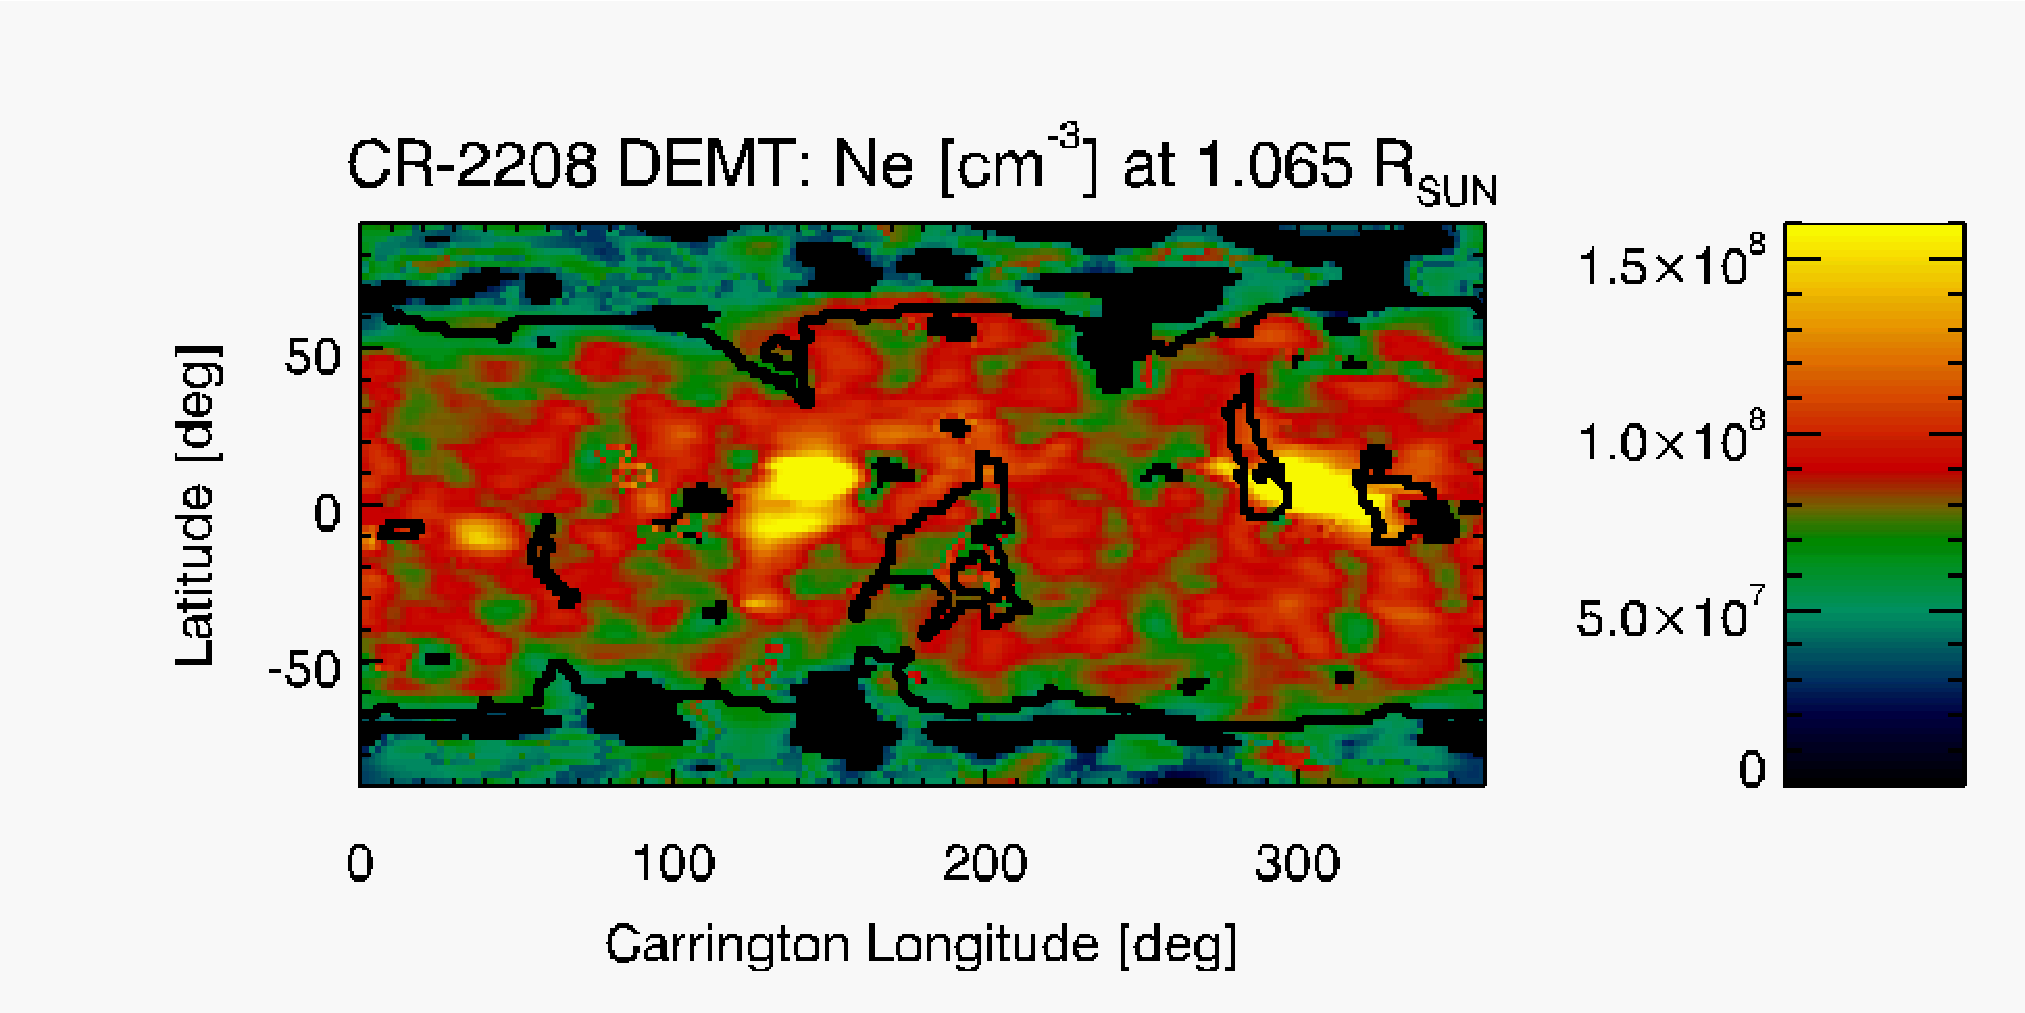
\includegraphics[width=0.495\textwidth]{figs/map_Ne_CR2208_DEMT-AIA_H1_L522_r3d_1065_Rsun.pdf}
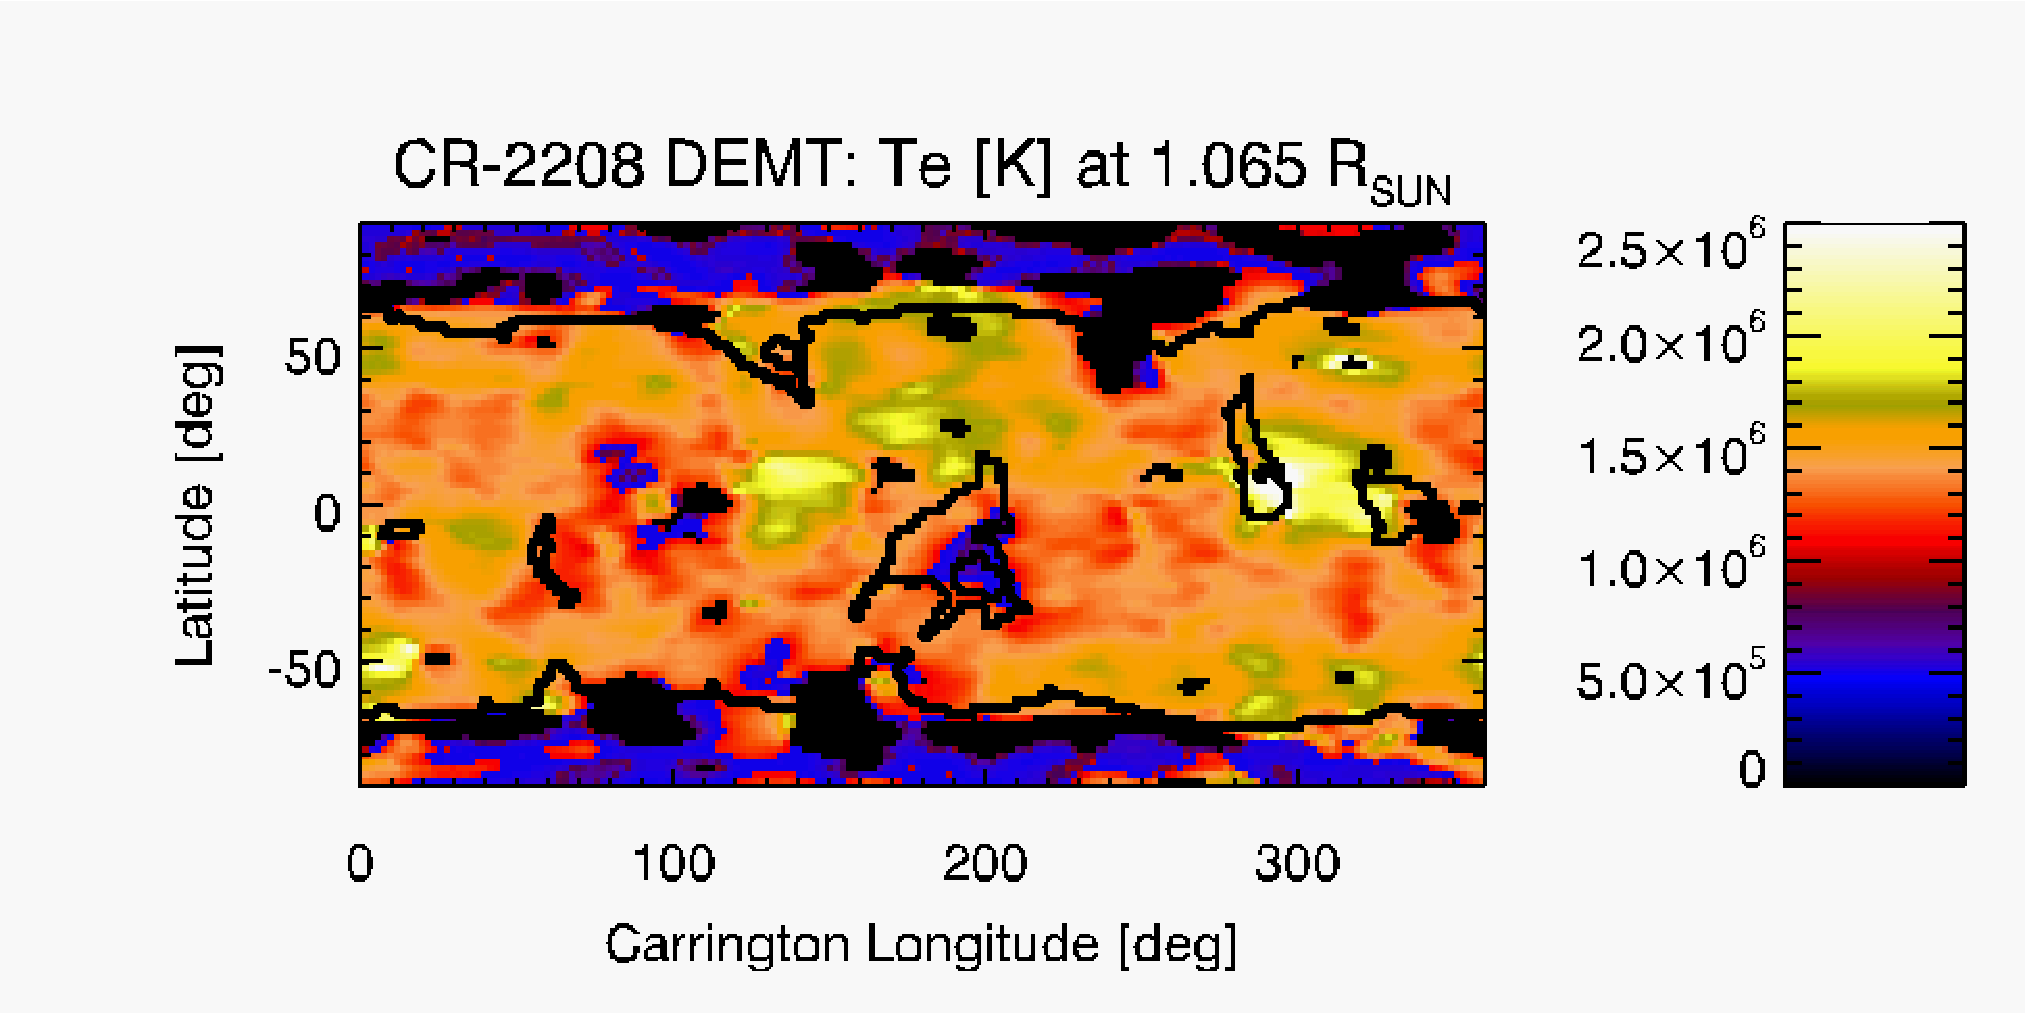
\includegraphics[width=0.495\textwidth]{figs/map_Tm_CR2208_DEMT-AIA_H1_L522_r3d_1065_Rsun.pdf}
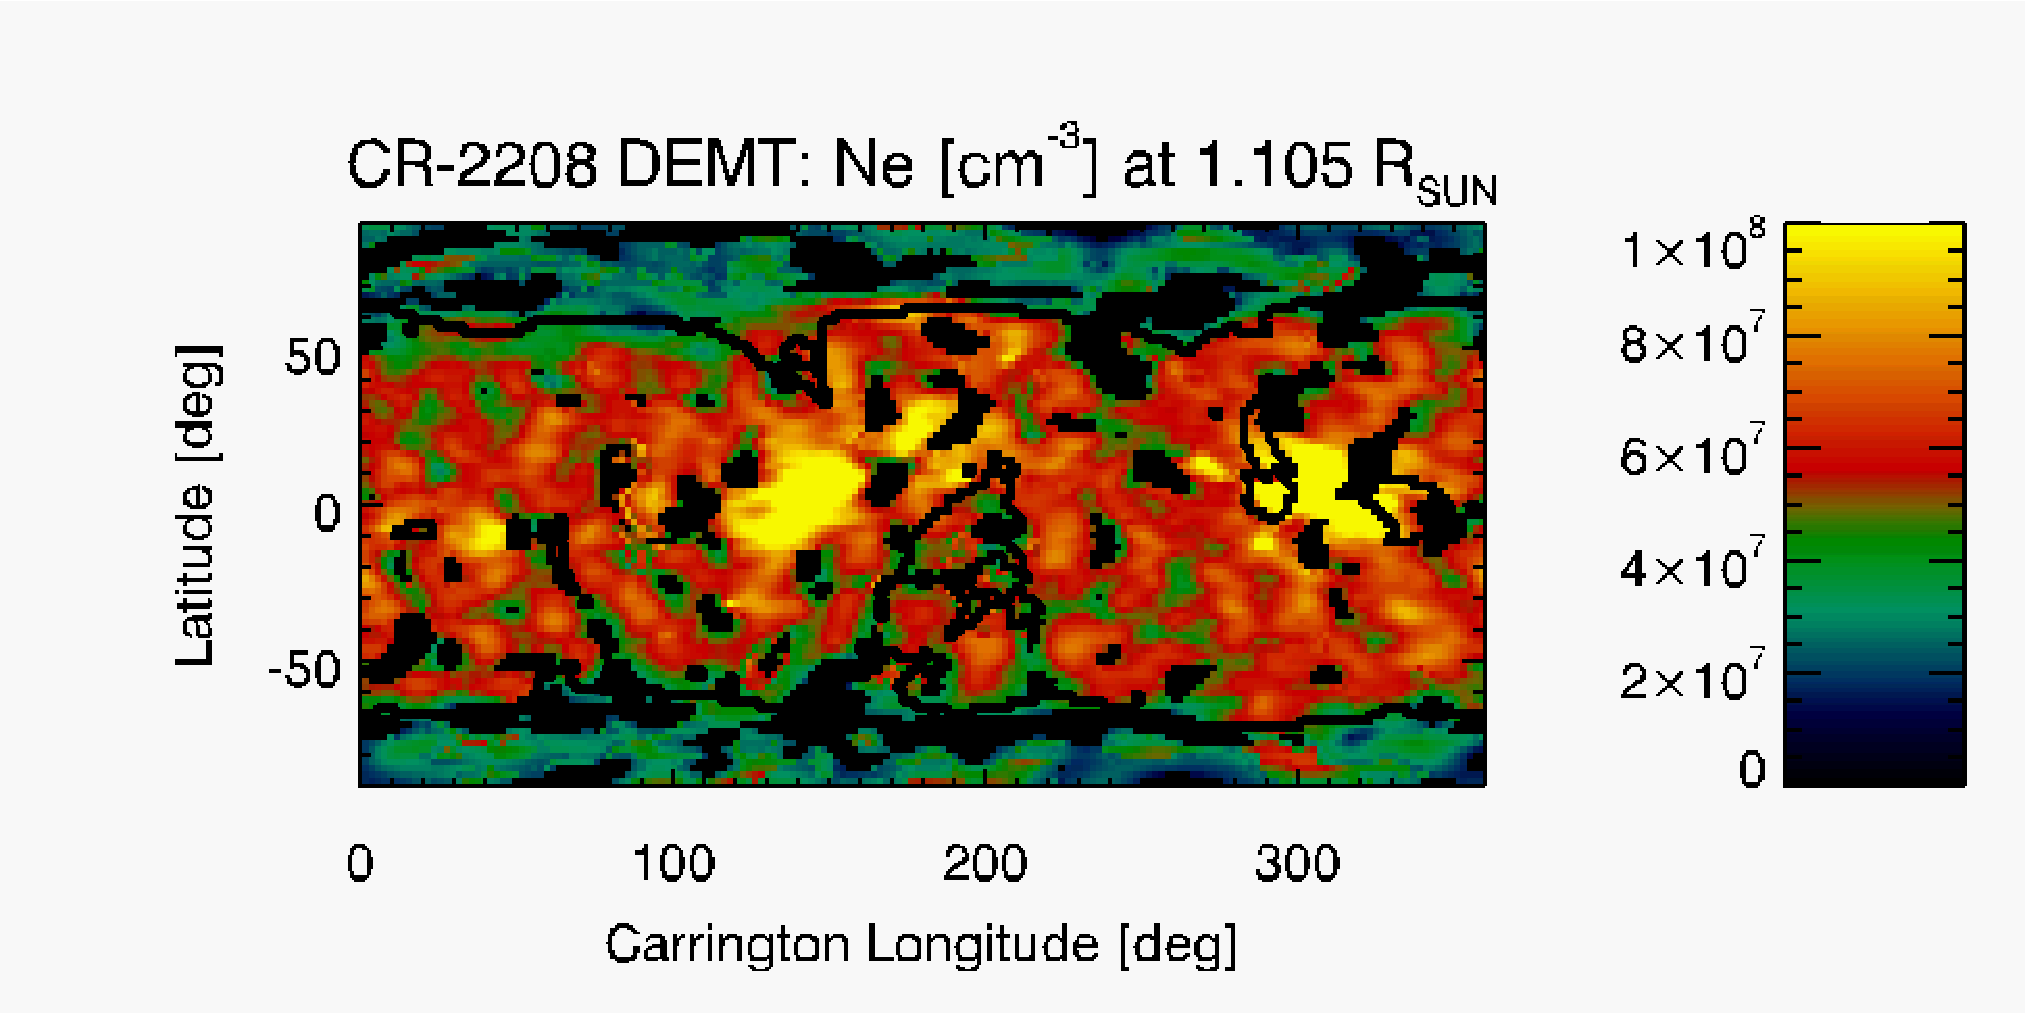
\includegraphics[width=0.495\textwidth]{figs/map_Ne_CR2208_DEMT-AIA_H1_L522_r3d_1105_Rsun.pdf}
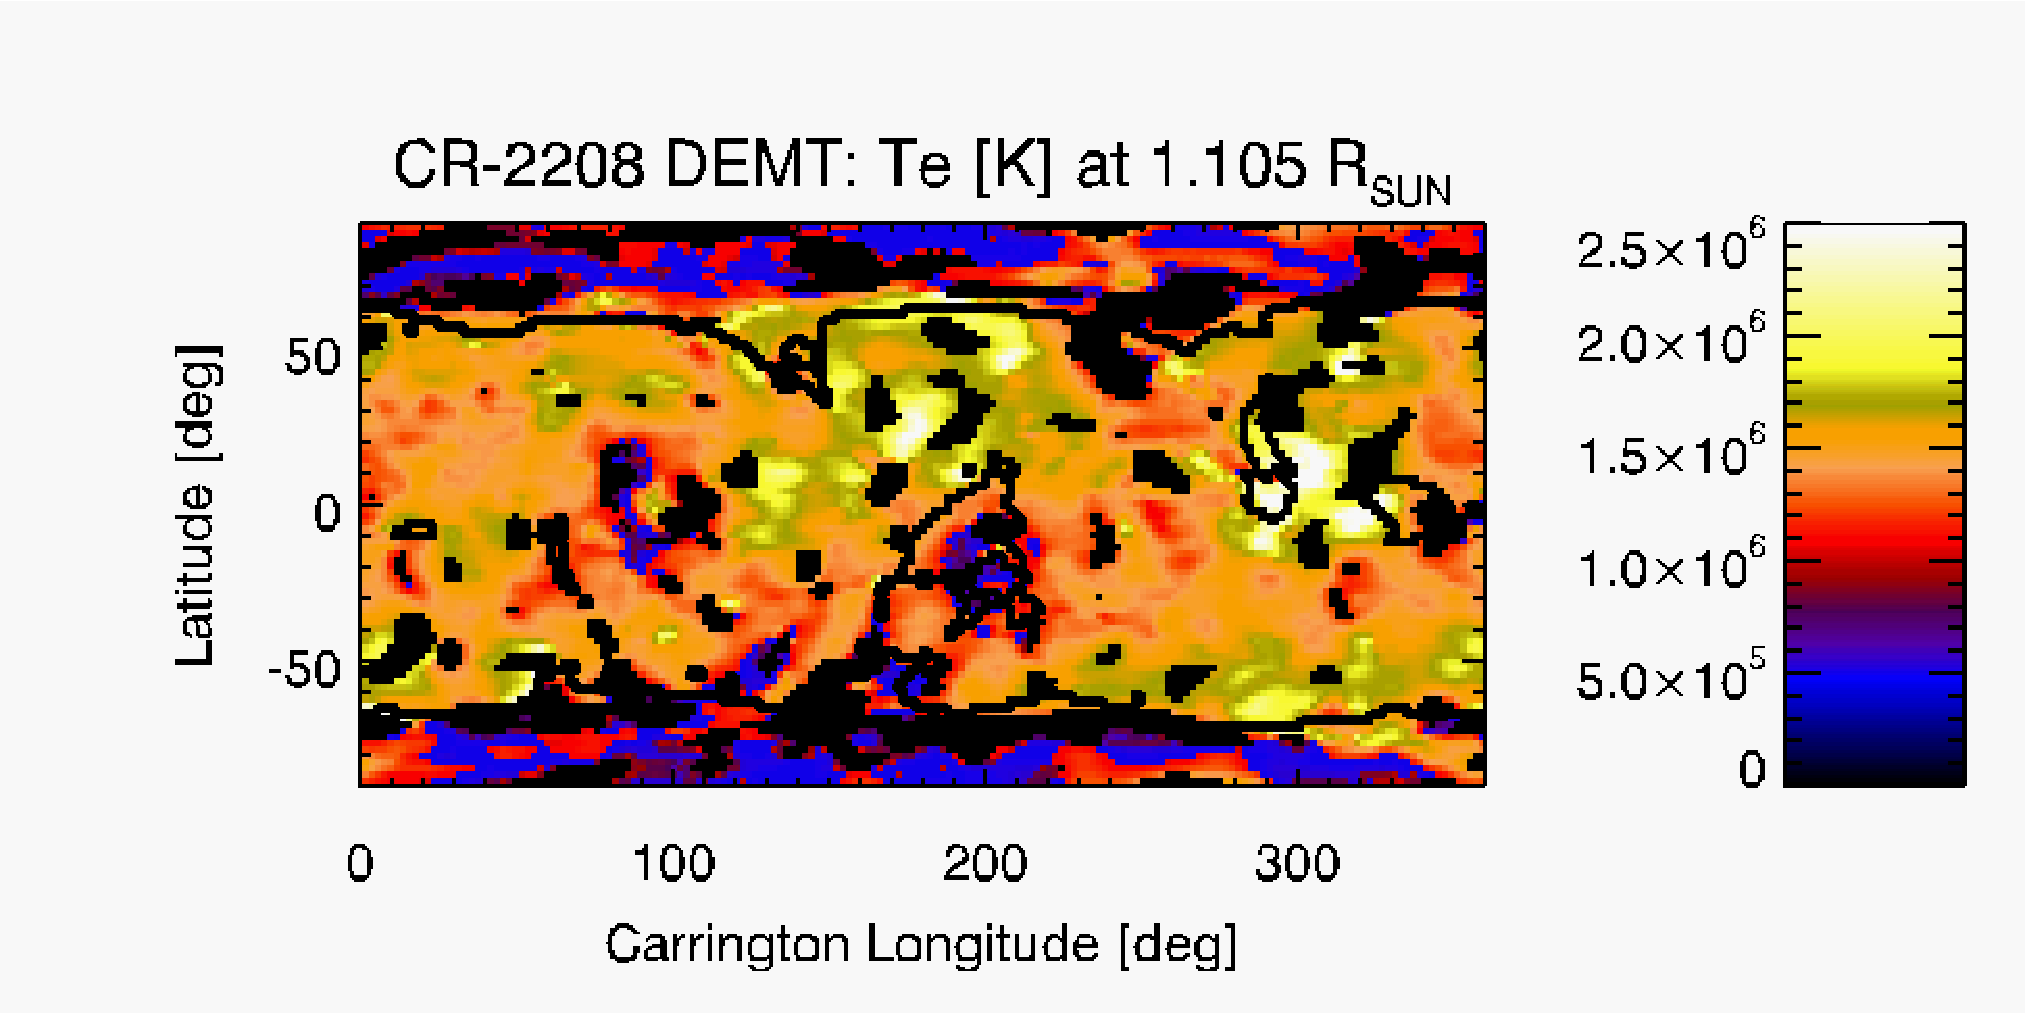
\includegraphics[width=0.495\textwidth]{figs/map_Tm_CR2208_DEMT-AIA_H1_L522_r3d_1105_Rsun.pdf}
\caption{Same as Figure \ref{carmaps_demt_2082} but for CR-2208.}
\label{carmaps_demt_2208}
\end{center}
\end{figure}



B)    I - Small-closed field lines. Small meaning with apex within the DEMT range of heights. This class thoroughly probes the inner core of the Streamer belt, where most of the DOWN loops showed up before, and will show up now.

  II - Large-closed field lines. Large meaning their apex surpasses the DEMT range of heights. This class is mostly populated by very large trans-equatorial field lines forming the "envelope" of the Streamer belt.

 III - Open field lines.

Carrington maps of the Lat/Lon location at 1.105 Rs of the field lines I (in blue), II (in red), and III (in green). This shows in a very graphical way which regions of the corona are probed by the three classes of selected field lines. 

\begin{figure}%[h]
\begin{center}
\includegraphics[width=0.495\textwidth,clip=]{figs/Highpoint_2082_demt_paper_Rpoint-map.eps}
%\includegraphics[width=0.495\textwidth,clip=]{Highpoint_2082_awsom_paper_Rpoint-map.eps}
\includegraphics[width=0.495\textwidth,clip=]{figs/Highpoint_2208_demt_paper_Rpoint-map.eps}
%\includegraphics[width=0.495\textwidth,clip=]{Highpoint_2208_awsom_paper_Rpoint-map.eps}
\caption{Latitude-longitude location of field lines meeting the criteria listed in Section \ref{trace} traced with DEMT results, at heights $1.105\,\mrsun$, for CR-2082(left panel) and CR-2208 (right panel). Different colors identify diverse thermodynamical and magnetic structures, as described in the text.}
\label{rpoint}
\end{center}
\end{figure} 



C) A plot of the average DEMT Ne(r) along all field lines of type I (in solid-blue), of type II (in solid-red and of type III (in solid-green). Over plotted in the same color code but in dashed-line style the AWSoM results along the same three statistical sample of field-lines. In particular, this shows the global 3D agreement between AWSoM and DEMT in distinct magnetic structures and carefully tracing along field lines 

D) Same as C) but for Te.

C) and D) will be complemented with companion histograms showing in a statistical fashion how AWSoM and DEMT results compare.

E) As the two rotations are strongly axis-symmetric we want to show the longitude-averaged results of DEMT at a low height, say 1.105 Rsun, along with AWSoM results. In the attached plot we show the DEMT and AWSoM longitude-averaged results at 1.105 Rsun in the top two panels (one for each rotation). The vertical lines indicate the longitude-averaged latitudes of the North and South OC boundary. The LOW panels show the longitude-averaged AWSoM wind speed Vr at 6 Rsun, where all field lines are open. The HCS location is indicated by the minimum of the speed curve. Everything to the South of the HCS maps down to the Southern OPEN region in the top panels, and the same for the Northern hemisphere. It is pretty obvious the ANTI-CORRELATION between the tomographic Ne at low heights (coronal source region of the wind) and the Vr.

This plot (E) has never been shown before and I believe it is a very nice result. There are of course previous studies on this, but this would be the first time this is evaluated with tomography. It is not the terminal speed, but it already shows the fast/slow components. We can show this, or we can go for more. Diego can QUANTIFY the correlation by carefully mapping all open field lines at 6 Rsun down to the DEMT region. He needs to code a bit more to achieve this goal, but we believe it is worth. With that tool done Diego can explore other terminal values of quantities of the AWSoM model and the DEMT results below (expansion factor maybe?). This will be nice to do also for the July-2-2019 Eclipse rotation that we will analyze after this paper. 




\subsection{Tomography and Models}\label{awsom_res} 

\begin{figure}%[ht!]
\begin{center}
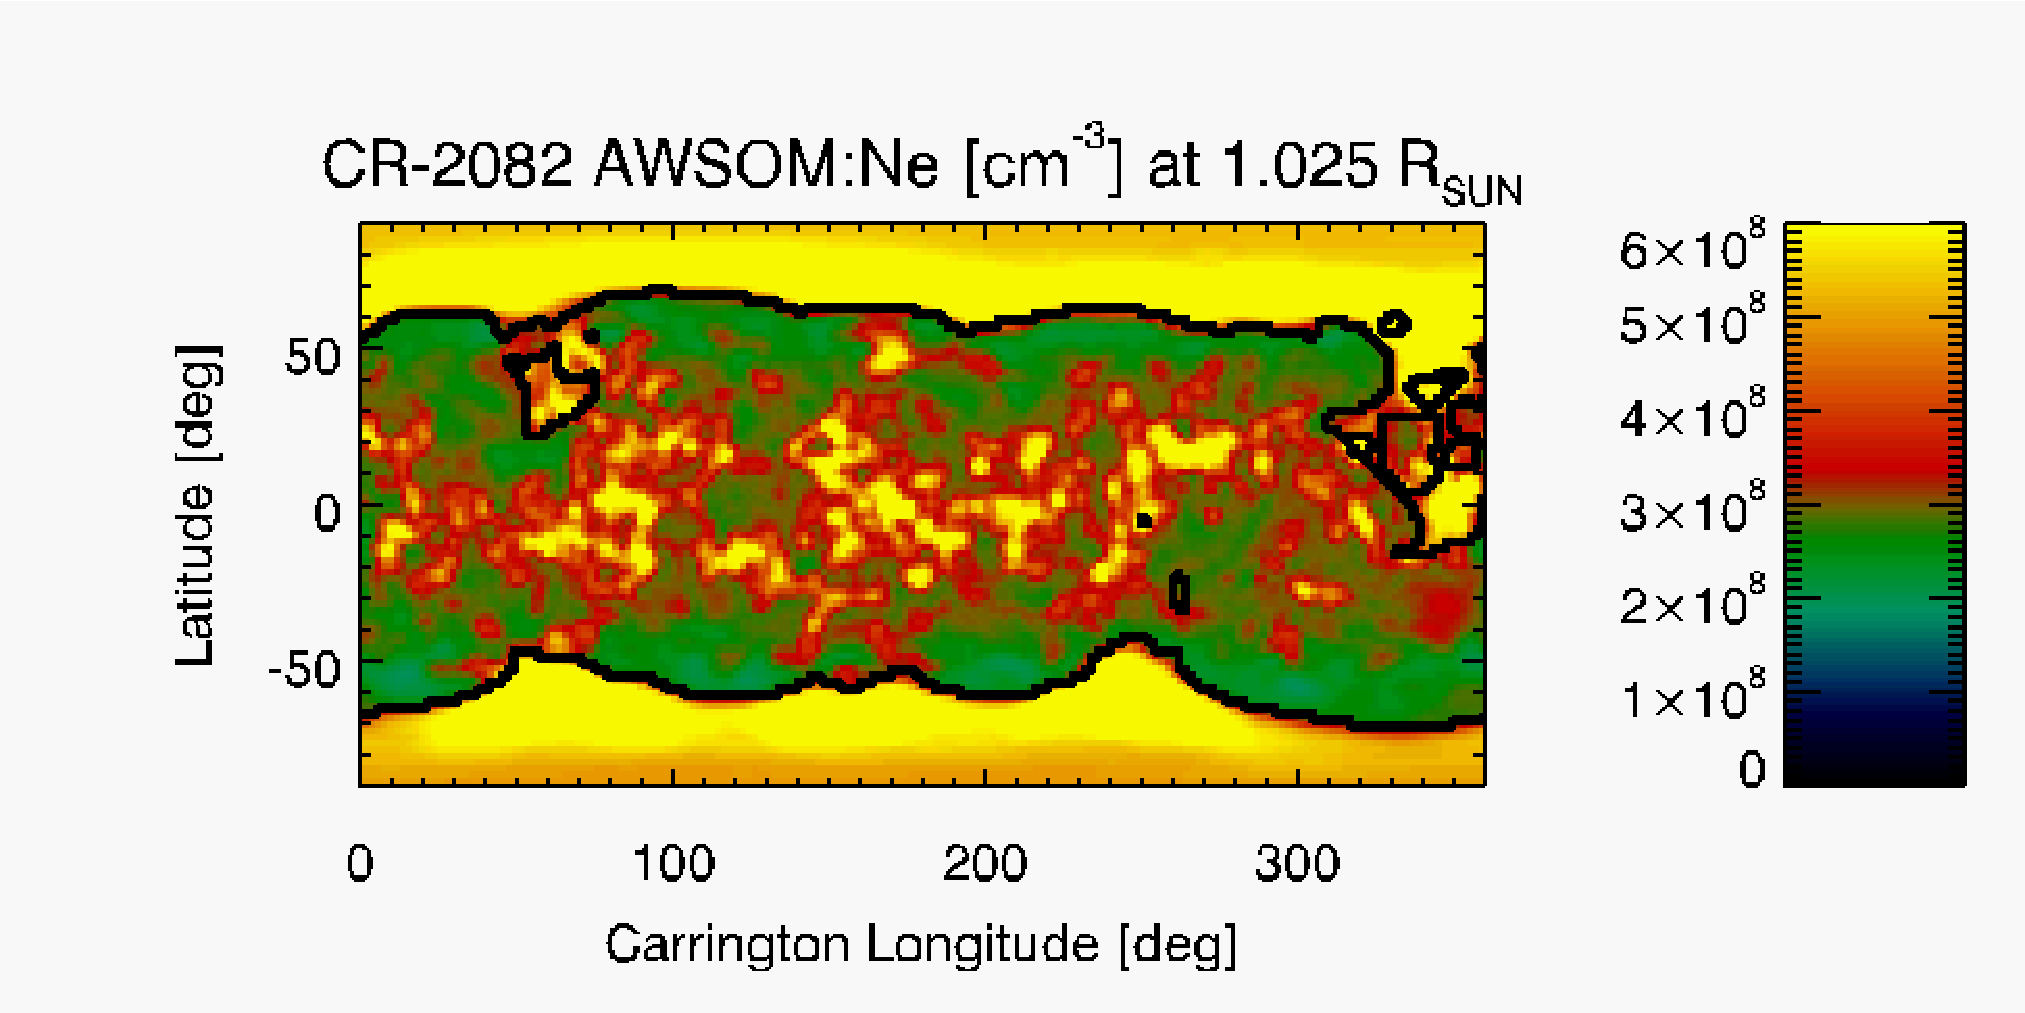
\includegraphics[width=0.495\textwidth]{figs/map_Ne_awsom_2082_185_short_1025_Rsun.pdf}
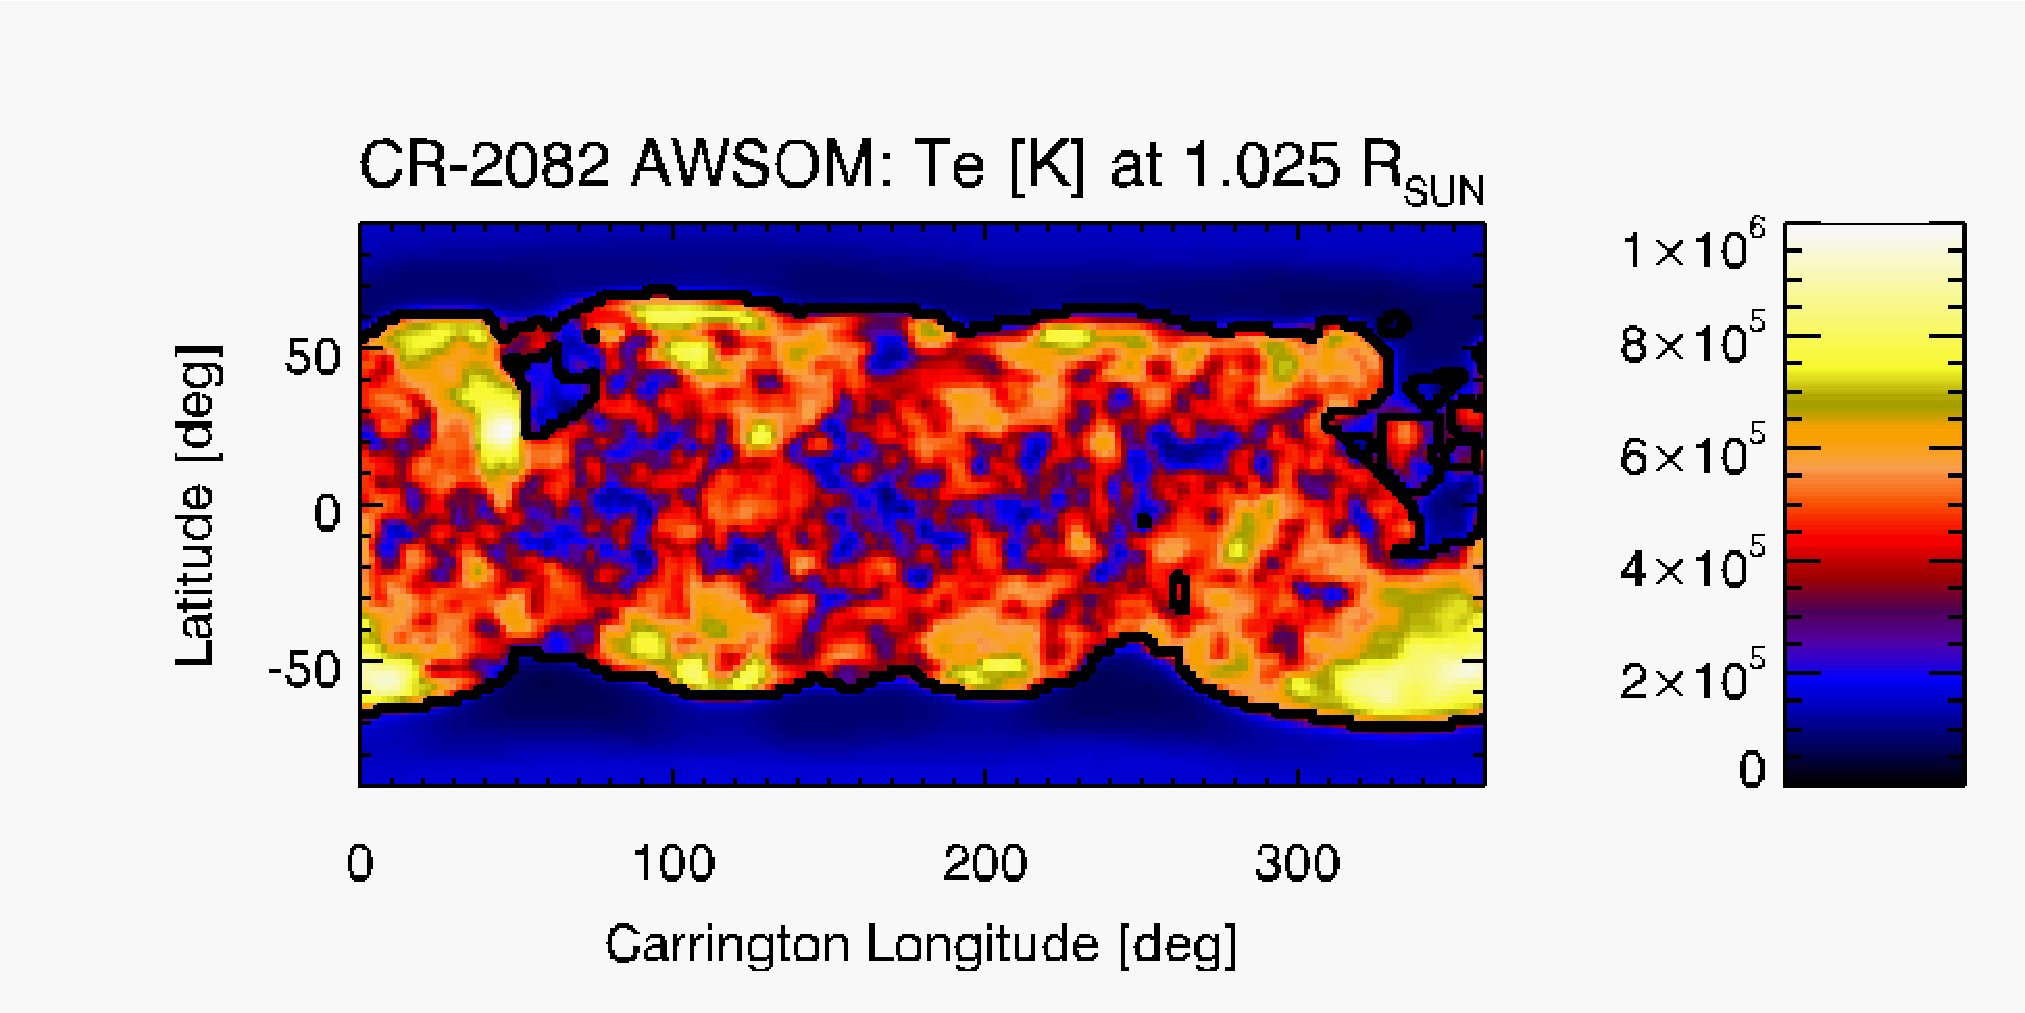
\includegraphics[width=0.495\textwidth]{figs/map_Te_awsom_2082_185_short_1025_Rsun.pdf}
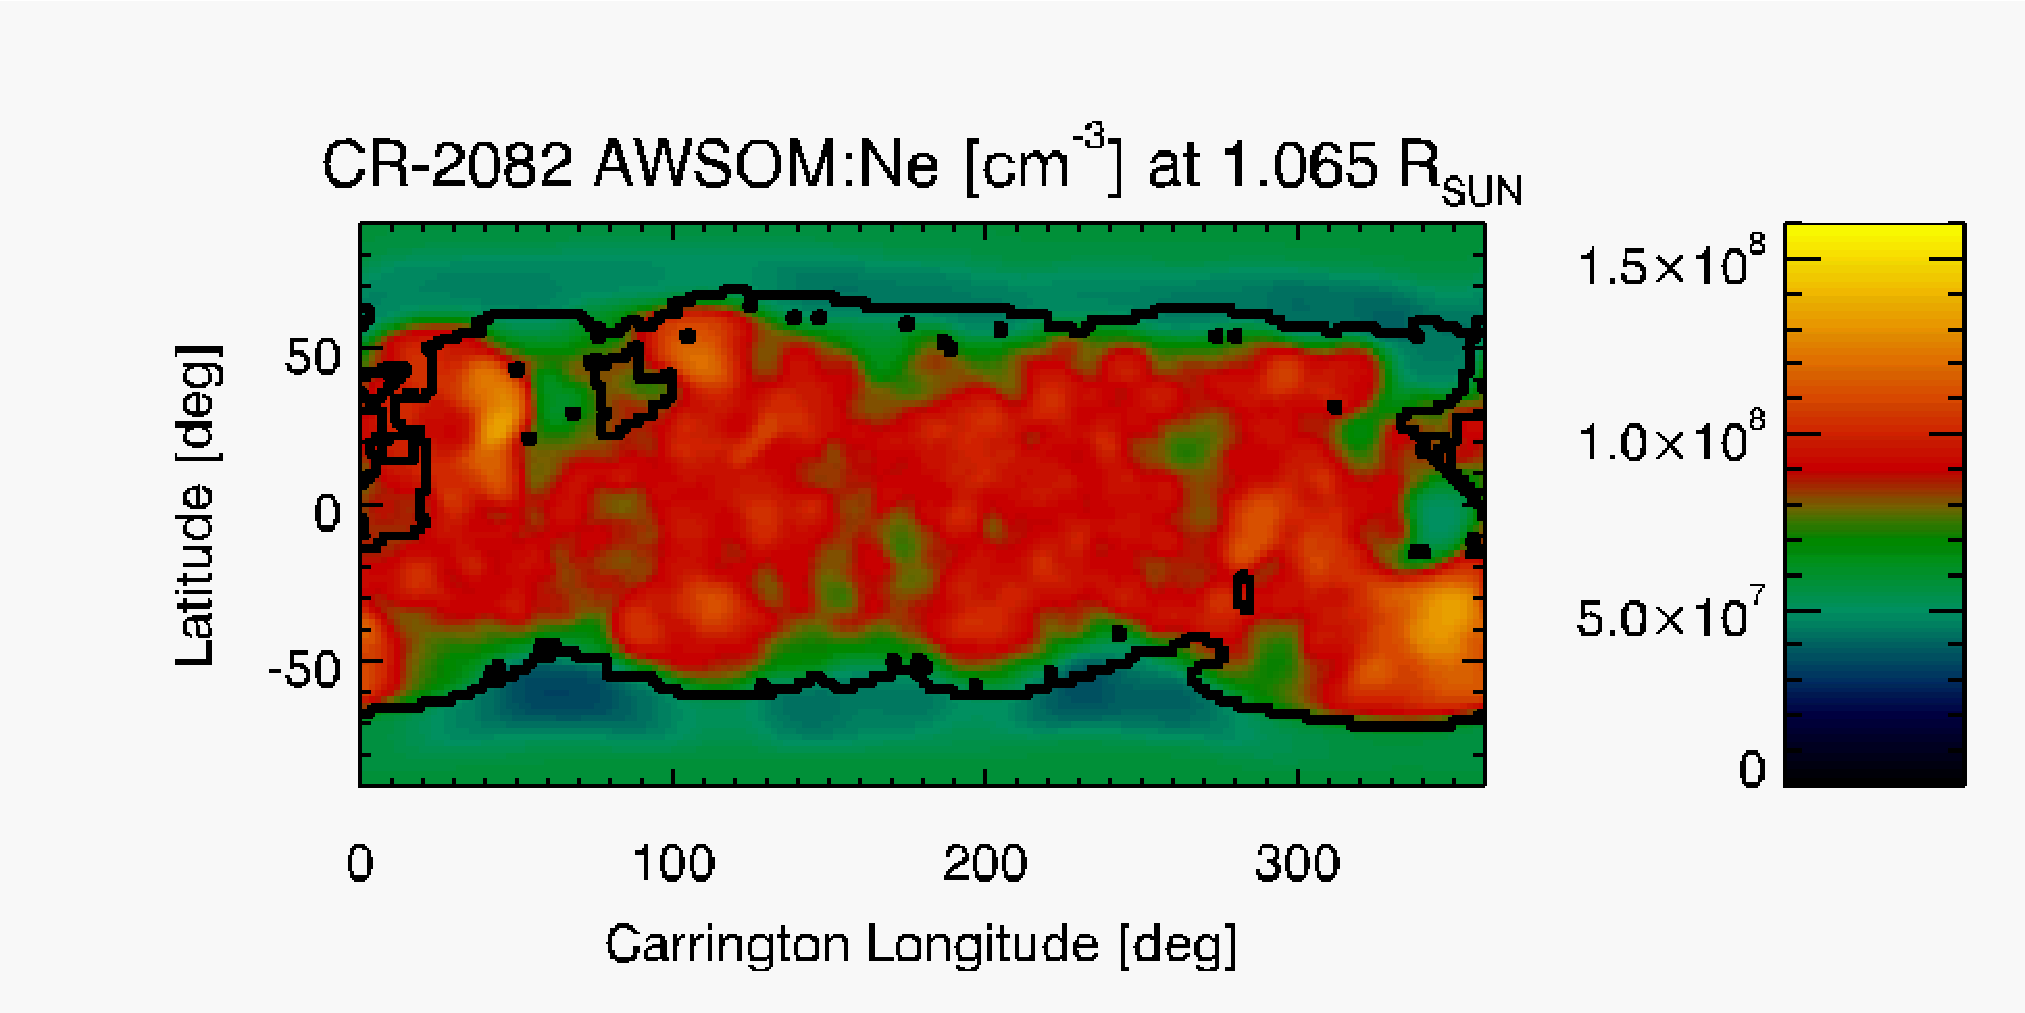
\includegraphics[width=0.495\textwidth]{figs/map_Ne_awsom_2082_185_short_1065_Rsun.pdf}
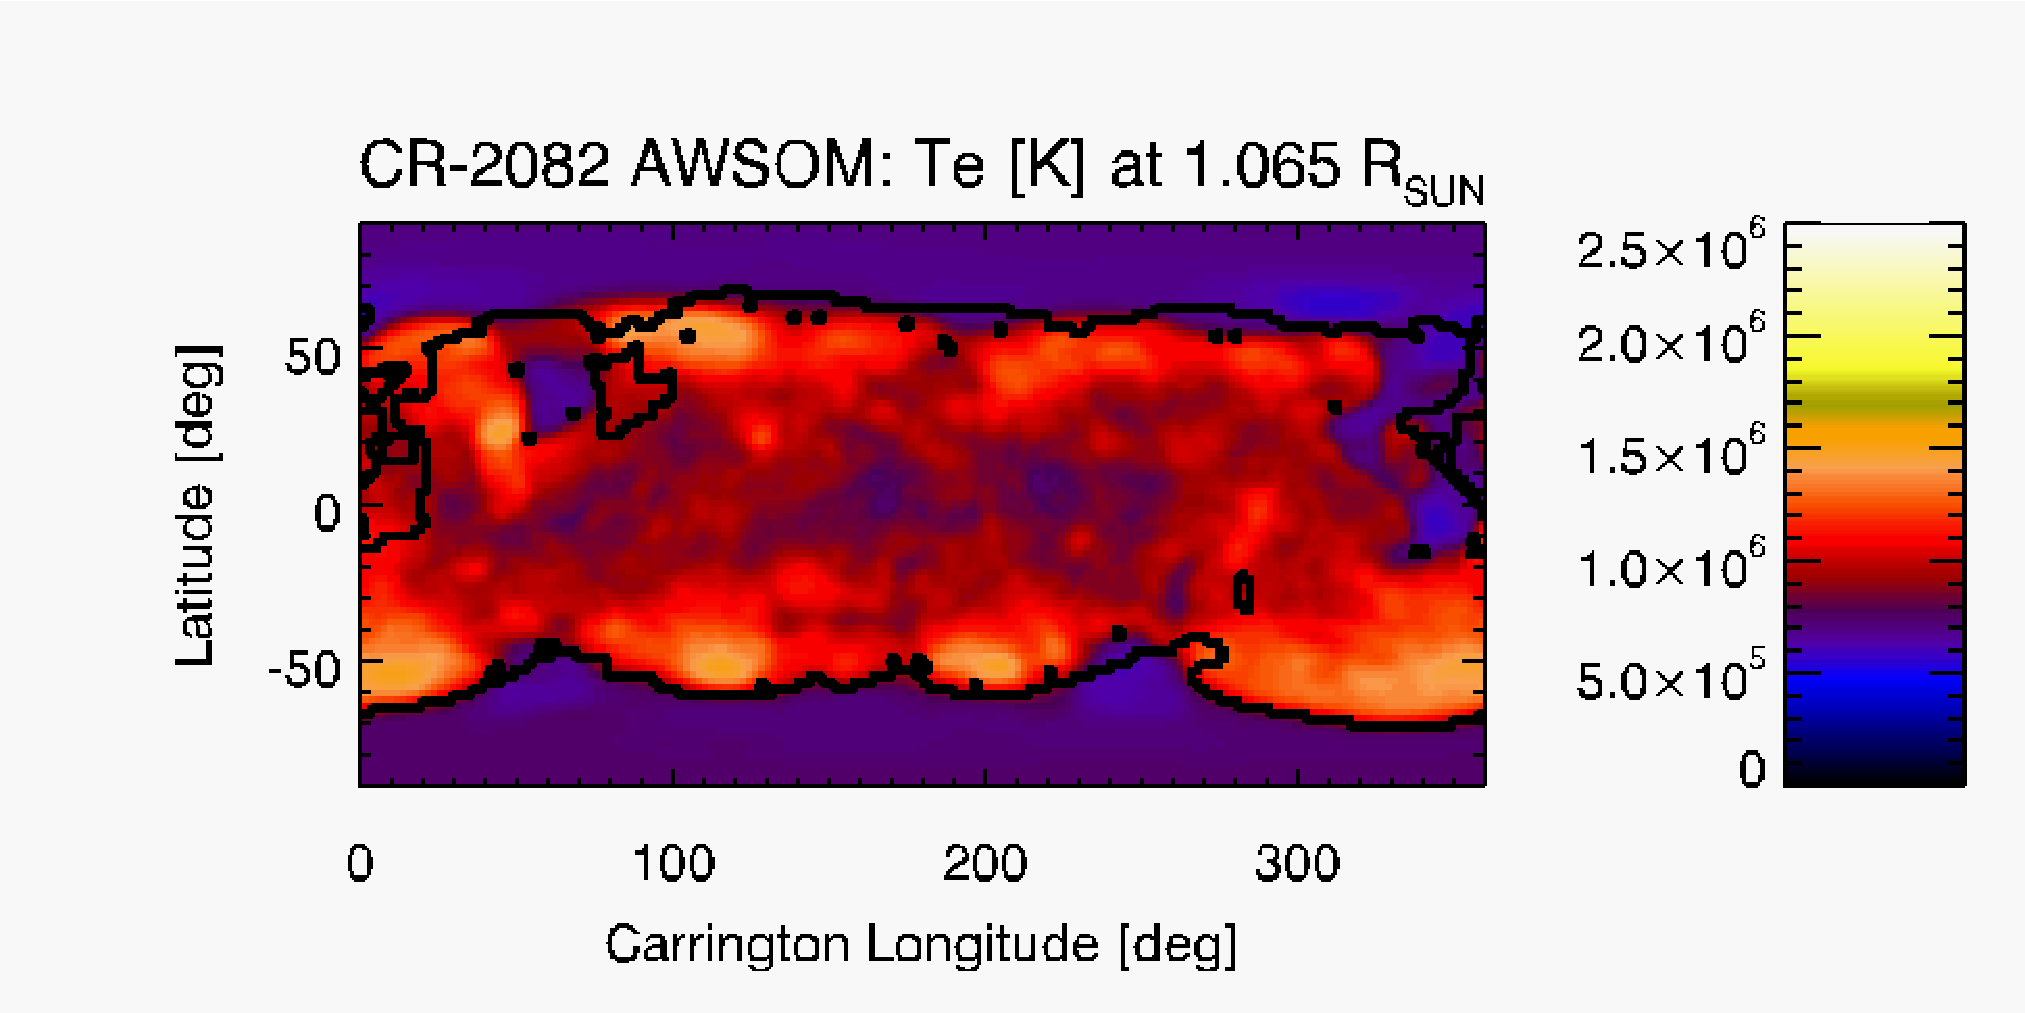
\includegraphics[width=0.495\textwidth]{figs/map_Te_awsom_2082_185_short_1065_Rsun.pdf}
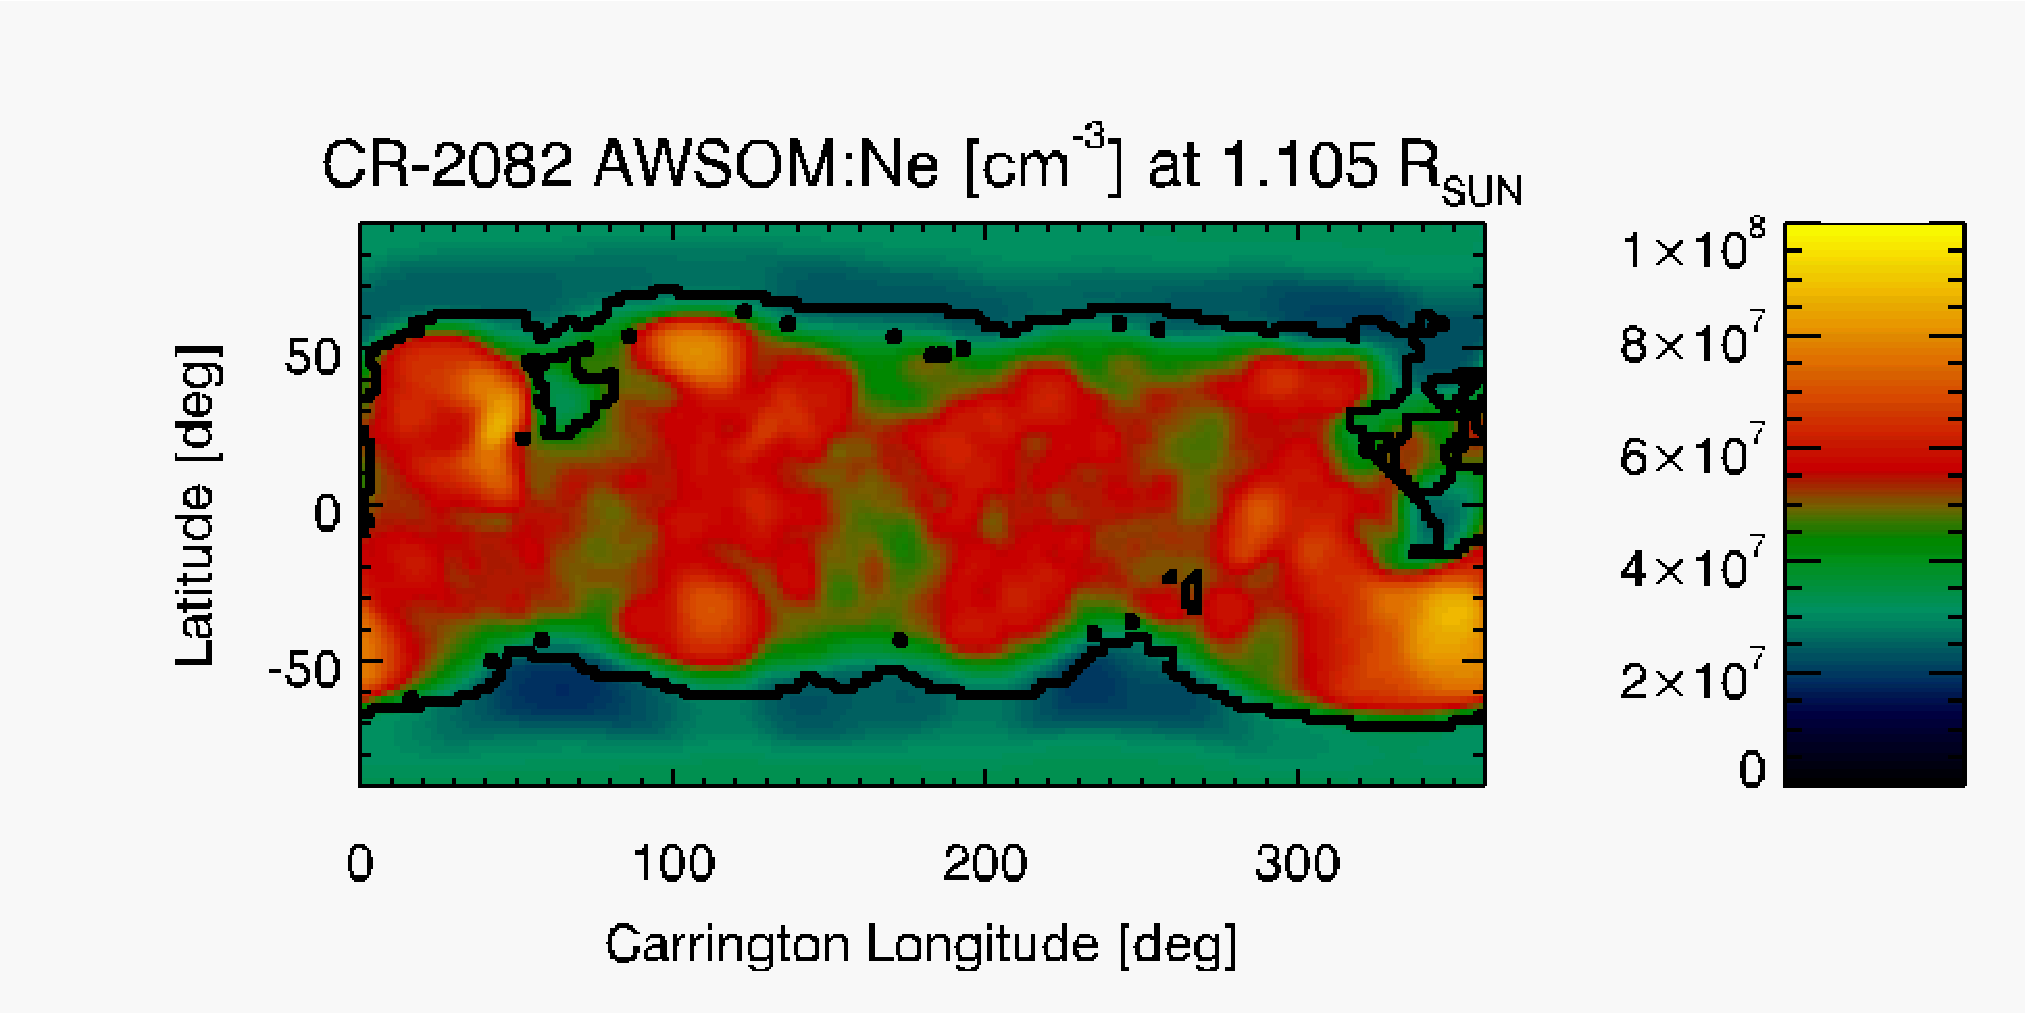
\includegraphics[width=0.495\textwidth]{figs/map_Ne_awsom_2082_185_short_1105_Rsun.pdf}
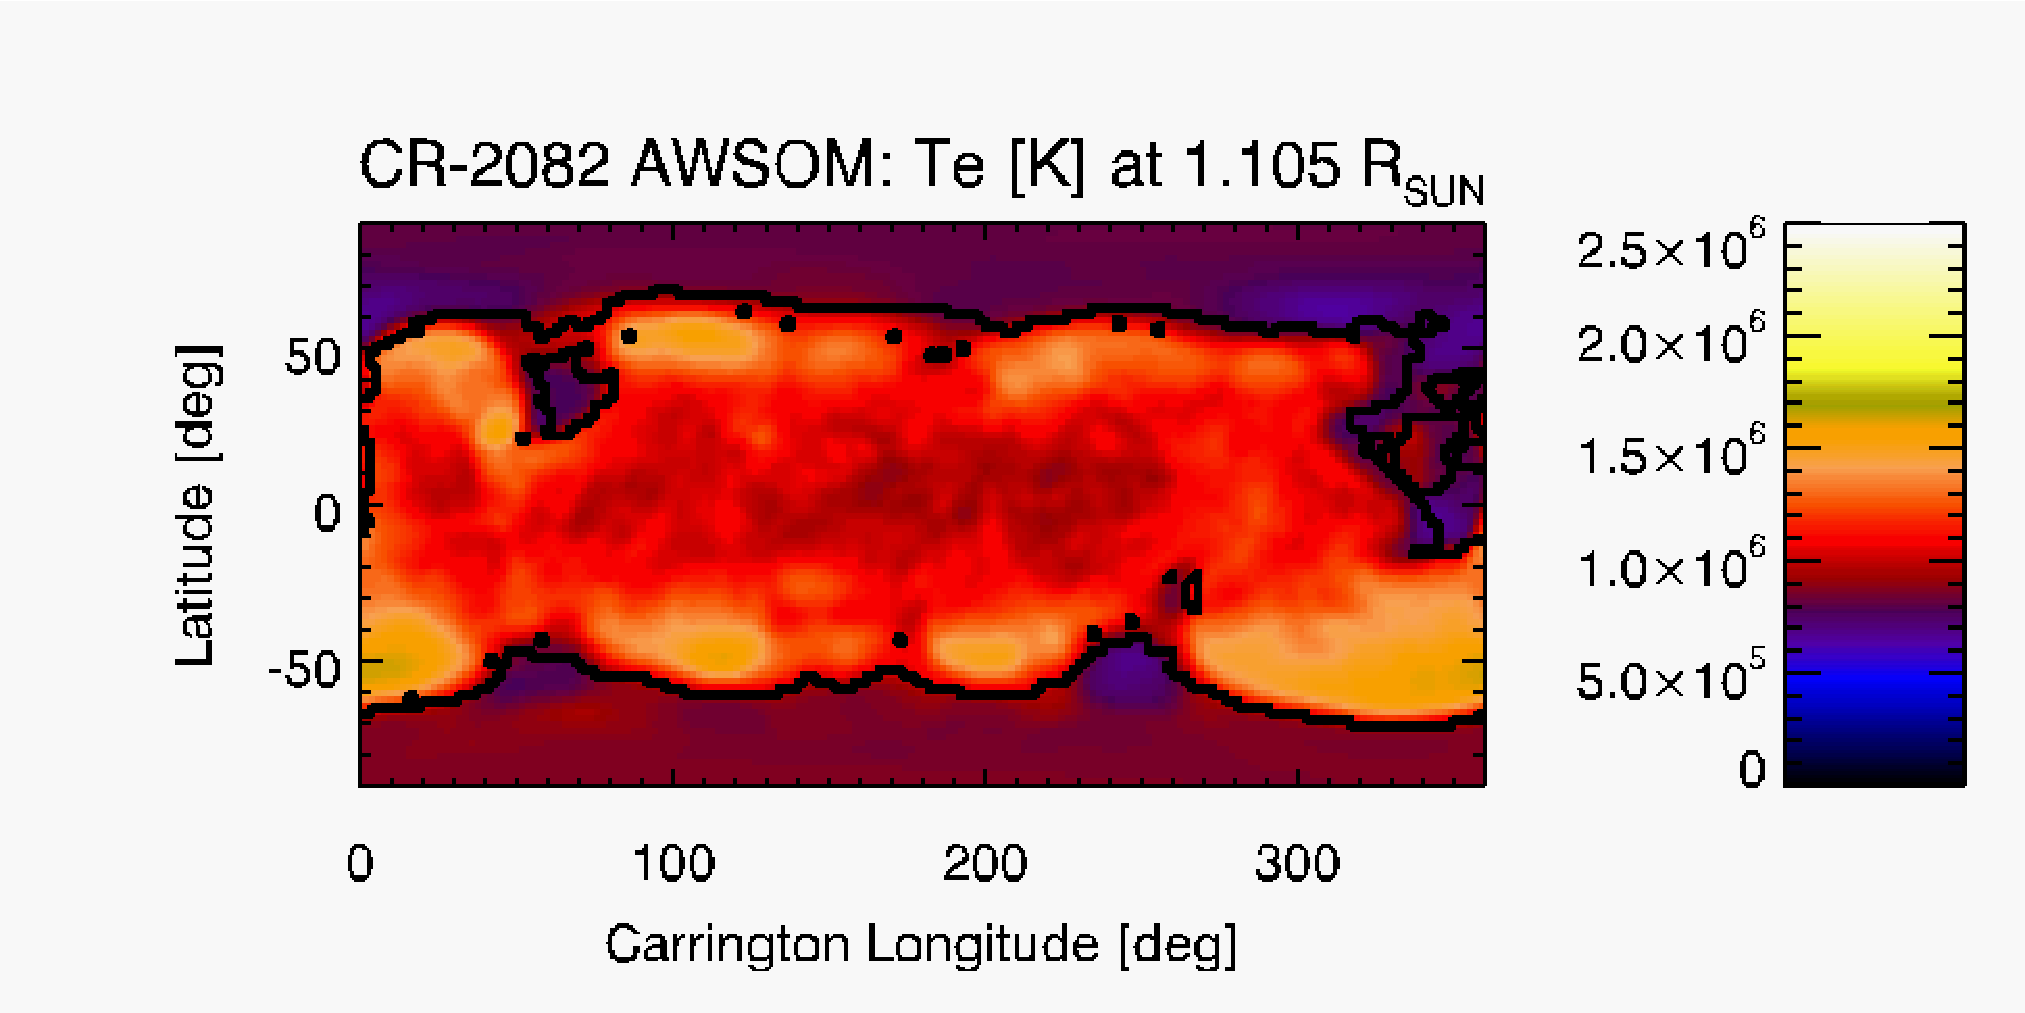
\includegraphics[width=0.495\textwidth]{figs/map_Te_awsom_2082_185_short_1105_Rsun.pdf}
\caption{Same as Figure \ref{carmaps_demt_2082} but for AWSoM results.}
\label{carmaps_awsom_2082}
\end{center}
\end{figure}

\begin{figure}%[ht!]
\begin{center}
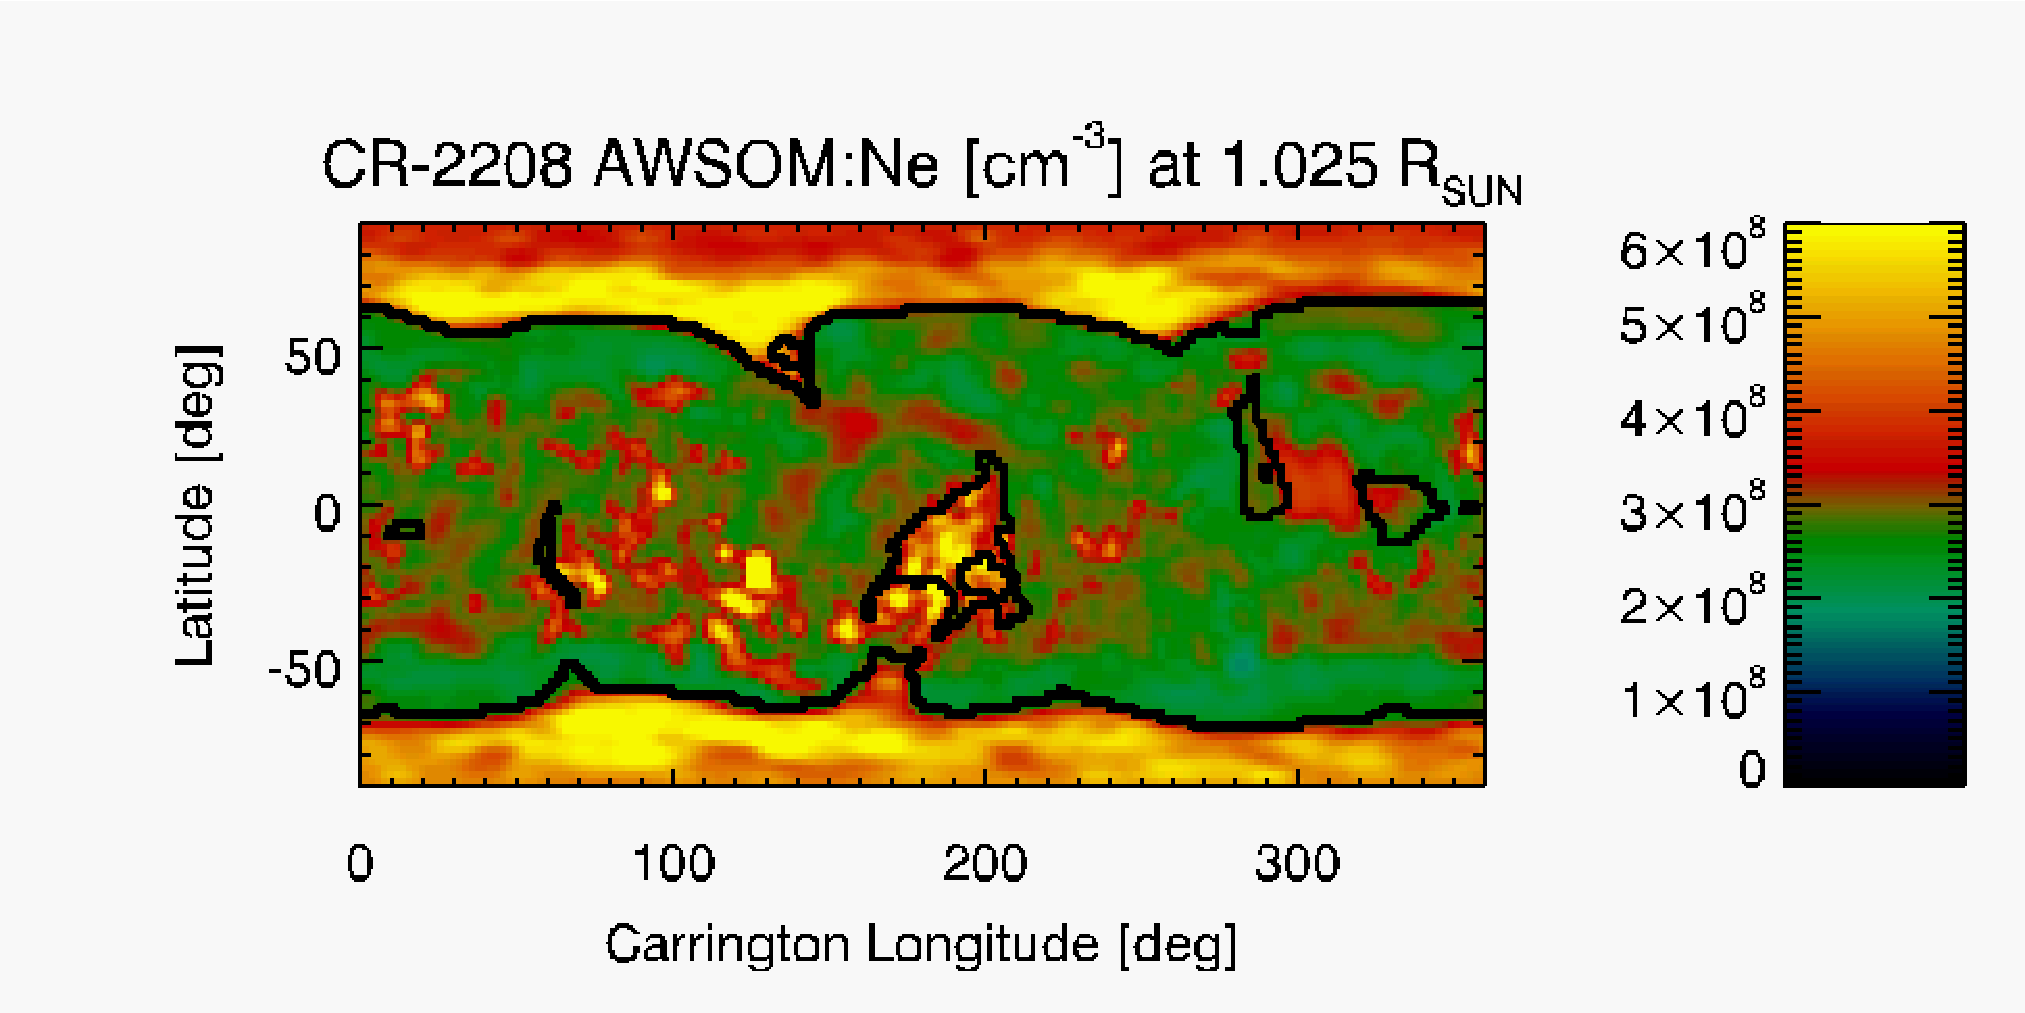
\includegraphics[width=0.495\textwidth]{figs/map_Ne_awsom_2208_185_short_1025_Rsun.pdf}
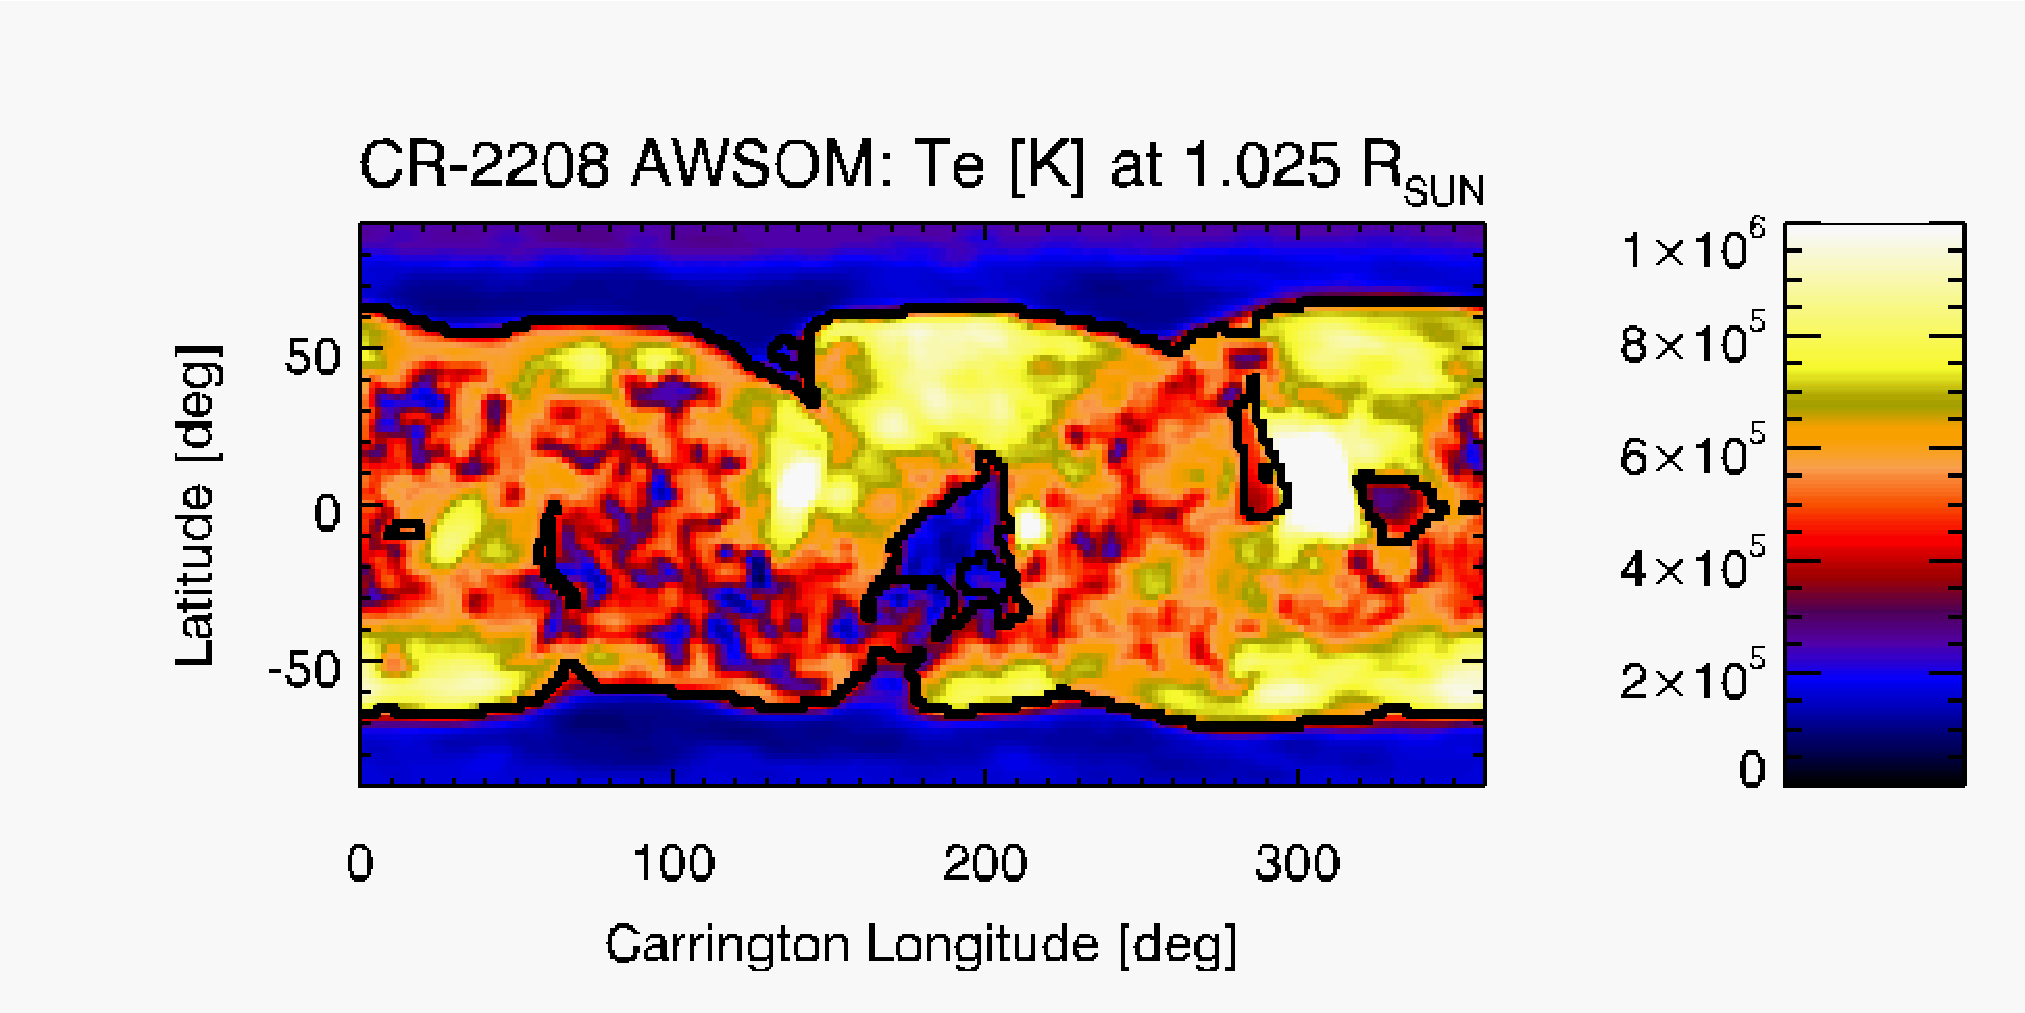
\includegraphics[width=0.495\textwidth]{figs/map_Te_awsom_2208_185_short_1025_Rsun.pdf}
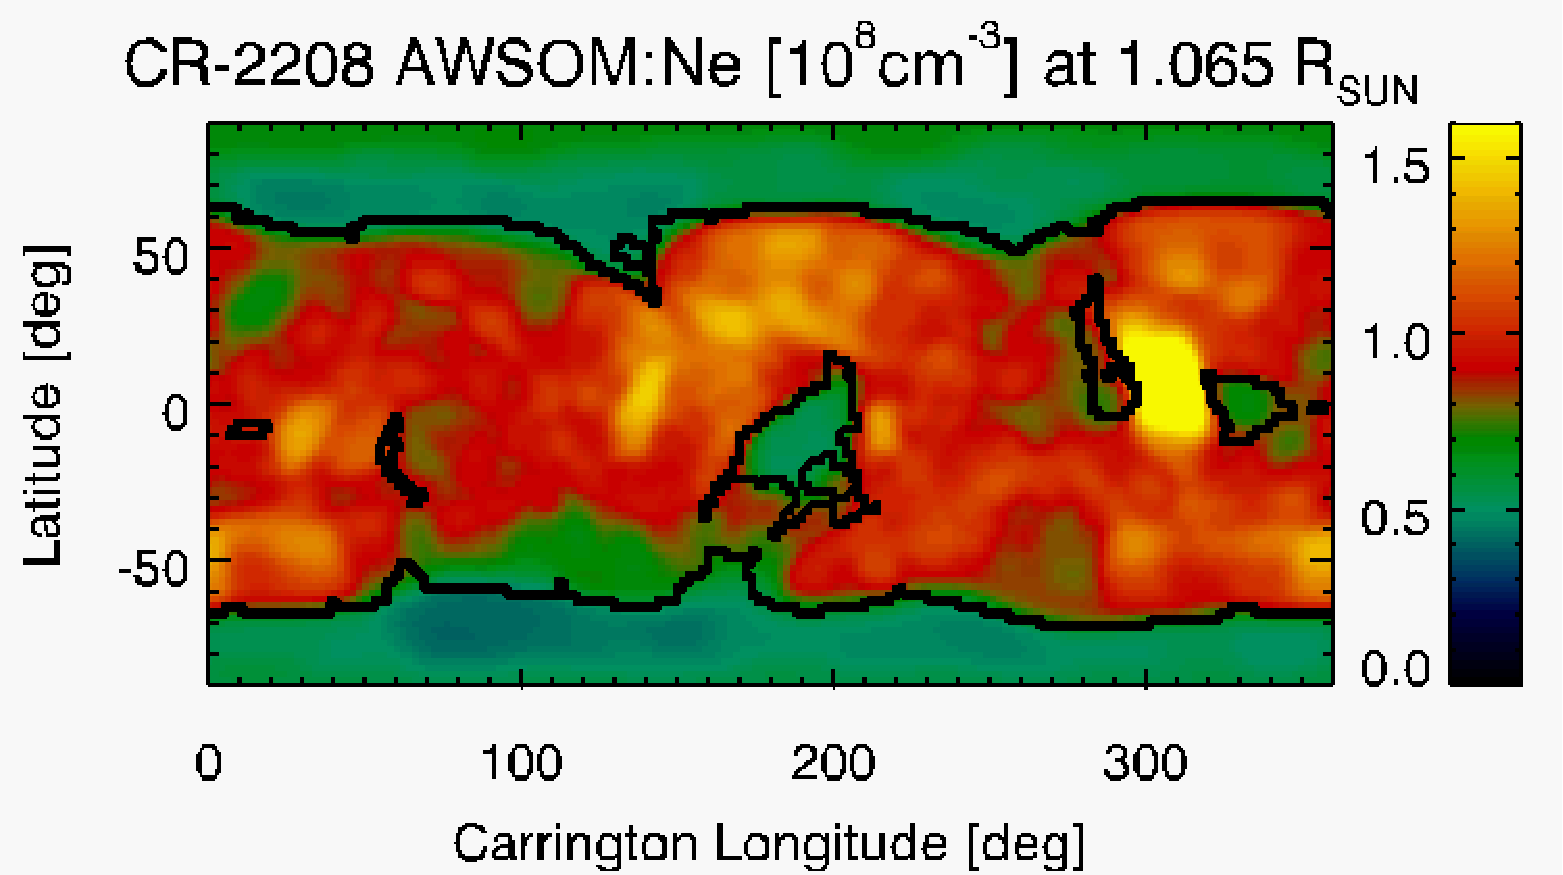
\includegraphics[width=0.495\textwidth]{figs/map_Ne_awsom_2208_185_short_1065_Rsun.pdf}
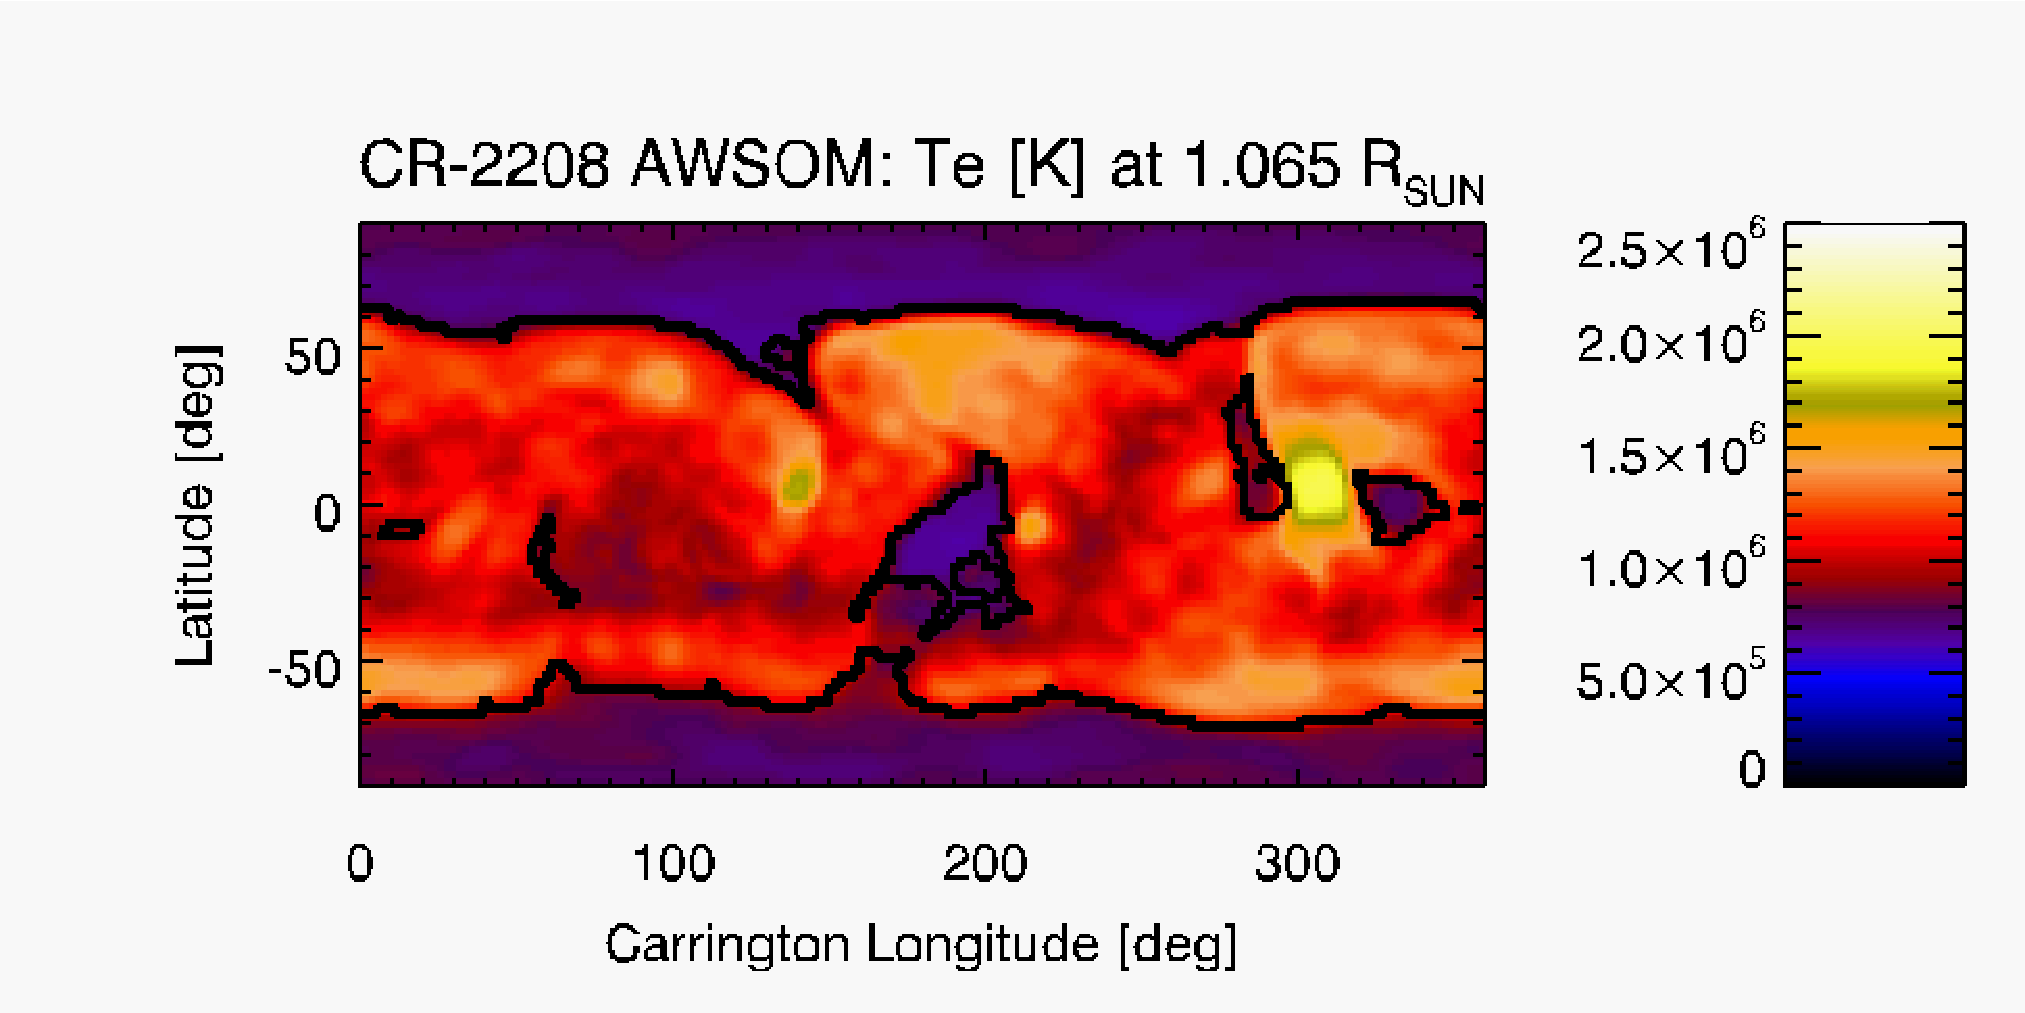
\includegraphics[width=0.495\textwidth]{figs/map_Te_awsom_2208_185_short_1065_Rsun.pdf}
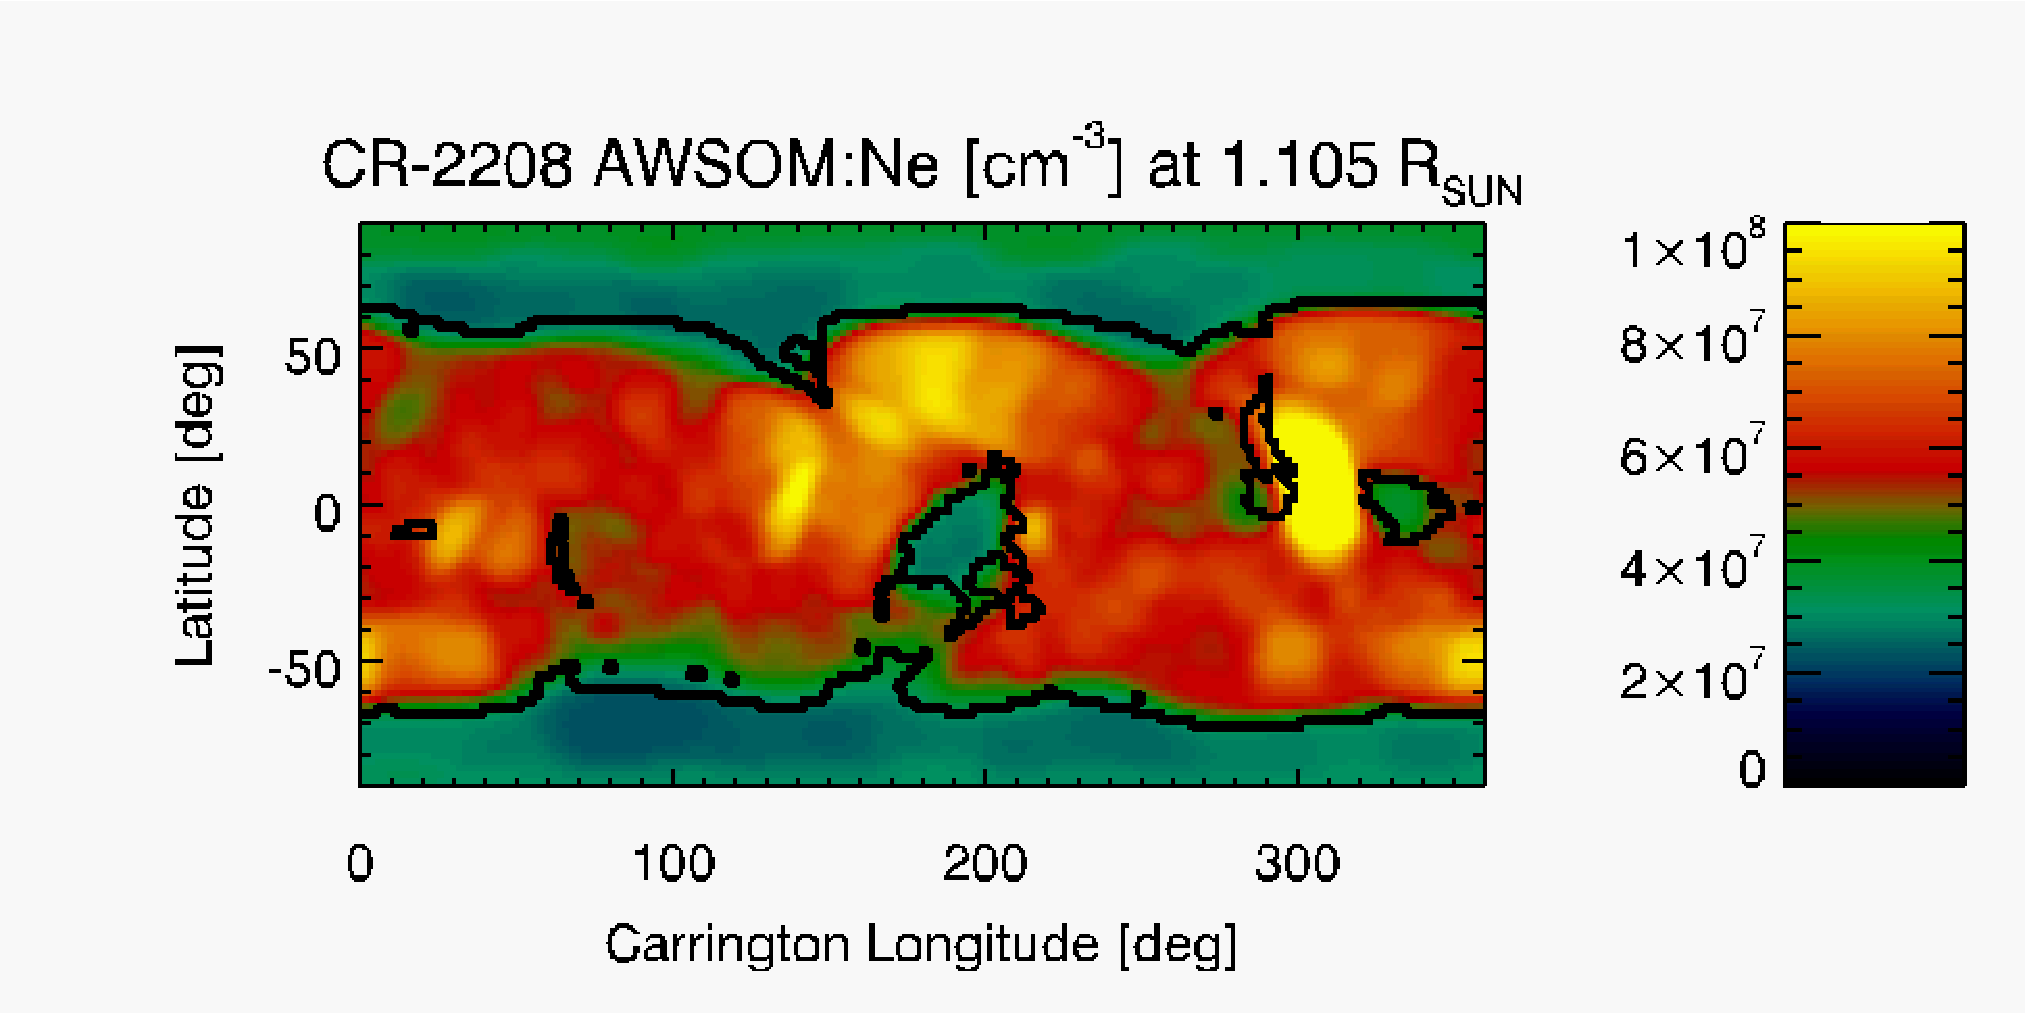
\includegraphics[width=0.495\textwidth]{figs/map_Ne_awsom_2208_185_short_1105_Rsun.pdf}
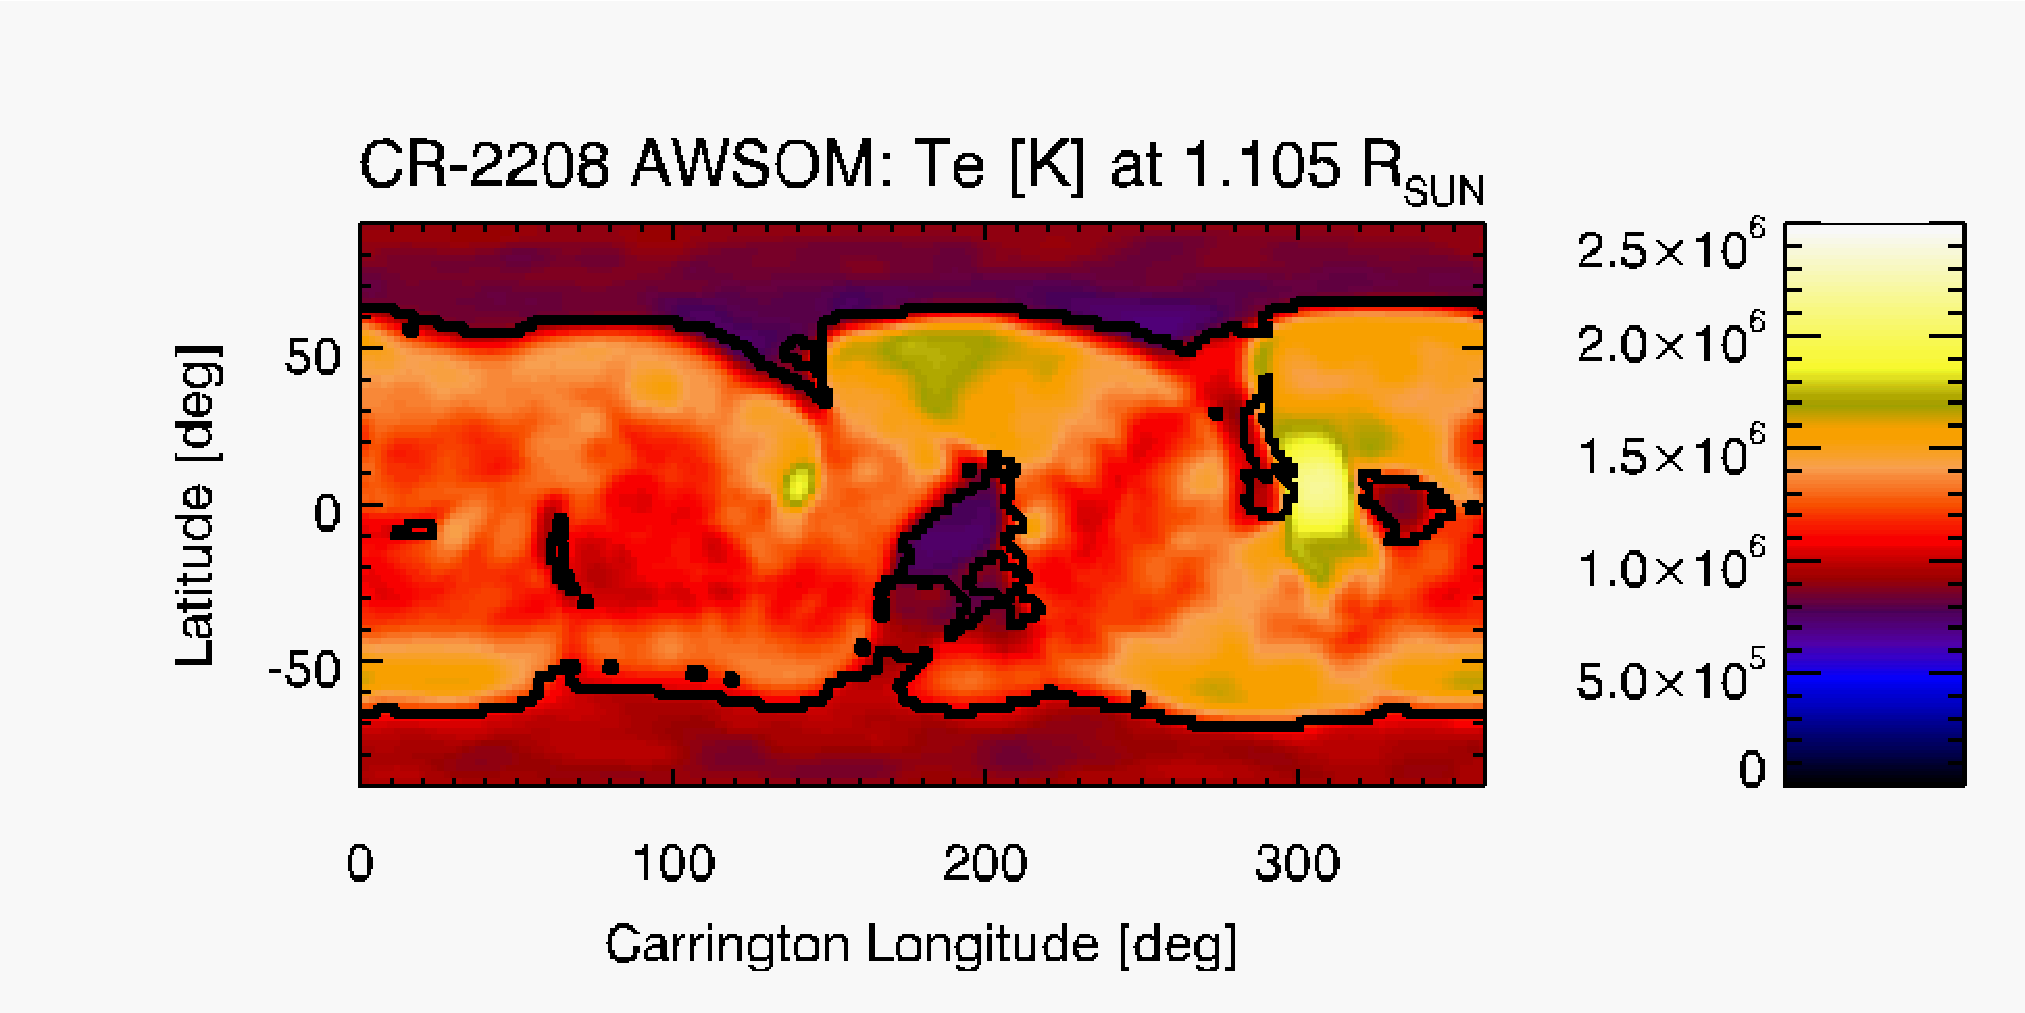
\includegraphics[width=0.495\textwidth]{figs/map_Te_awsom_2208_185_short_1105_Rsun.pdf}
\caption{Same as Figure \ref{carmaps_demt_2208} but for AWSoM results.}
\label{carmaps_awsom_2208}
\end{center}
\end{figure}

\begin{figure}%[h]
\begin{center}
%\includegraphics[width=0.495\textwidth,clip=]{Highpoint_2082_demt_paper_Rpoint-map.eps}
\includegraphics[width=0.495\textwidth,clip=]{figs/Highpoint_2082_awsom_paper_Rpoint-map.eps}
%\includegraphics[width=0.495\textwidth,clip=]{Highpoint_2208_demt_paper_Rpoint-map.eps}
\includegraphics[width=0.495\textwidth,clip=]{figs/Highpoint_2208_awsom_paper_Rpoint-map.eps}
\caption{Same as \ref{rpoint_demt} but for AWSoM loops.}
\label{rpoint_awsom}
\end{center}
\end{figure} 


\section{Discussion}\label{discu} 
%% Figure 
%
% \begin{figure} 
% \centerline{\includegraphics[width=0.5\textwidth,clip=]{<fig.eps>}}
% \caption{}%\label{fig:?}
% \end{figure}



%% Table
%
% \begin{table}
% \caption{}%\label{tbl:?}
% \begin{tabular}{}     
% \hline
% \multicolumn{2}{c}{<>}
% <data>
% \hline
% \end{tabular}
% \end{table}
  

%%%%%%%%%%%%%%%%%%%%%%%%%%%%%%%%%%%%%%%%%%%%%%%%%%%%%%%%%%%%%%%%%%%%%%%%%%%
%% Appendix
%
% \appendix   



%%%%%%%%%%%%%%%%%%%%%%%%%%%%%%%%%%%%%%%%%%%%%%%%%%%%%%%%%%%%%%%%%%%%%%%%%%%
%% Acknowledgements
%
% \begin{acks}
%
% \end{acks}


%%% %%%%%%%%%%%%%%%%%%%%%%%%%%%%%%%%%%%%%%%%%%%%%%%%%%%%%%%%%%%
%% Bibliography
%
% Using BibTeX
%
% \bibliographystyle{spr-mp-sola}
% \bibliography{<bib file>}  
%
% Without BibTeX 
% \begin{thebibliography}{}
% \bibitem[\protect\citeauthoryear{Author}{Year}]{key}
%   <bibliographical entry>
%
% \bibitem[\protect\citeauthoryear{}{}]{}
%   
%  
% \end{thebibliography}

\end{article} 
\end{document}
